\section{Results and discussion}
\label{ch2:sec:results}

The proposed cases are used to control power flow of the ESMU using 24 days of uninterrupted sub-half-hourly load record.
At first, the time-series improvements are presented, where a day's peak reduction due to the sub-half-hourly schedule adjustment are highlighted.
Then, the daily peak reduction across the entire dataset is presented, following by a probability density plot to better compare these findings.
In the end, the ARX model's impact on the peak reduction performance is assessed.

\subsection{Time-series analysis}

\begin{figure}\centering
	\subfloat[]{%
		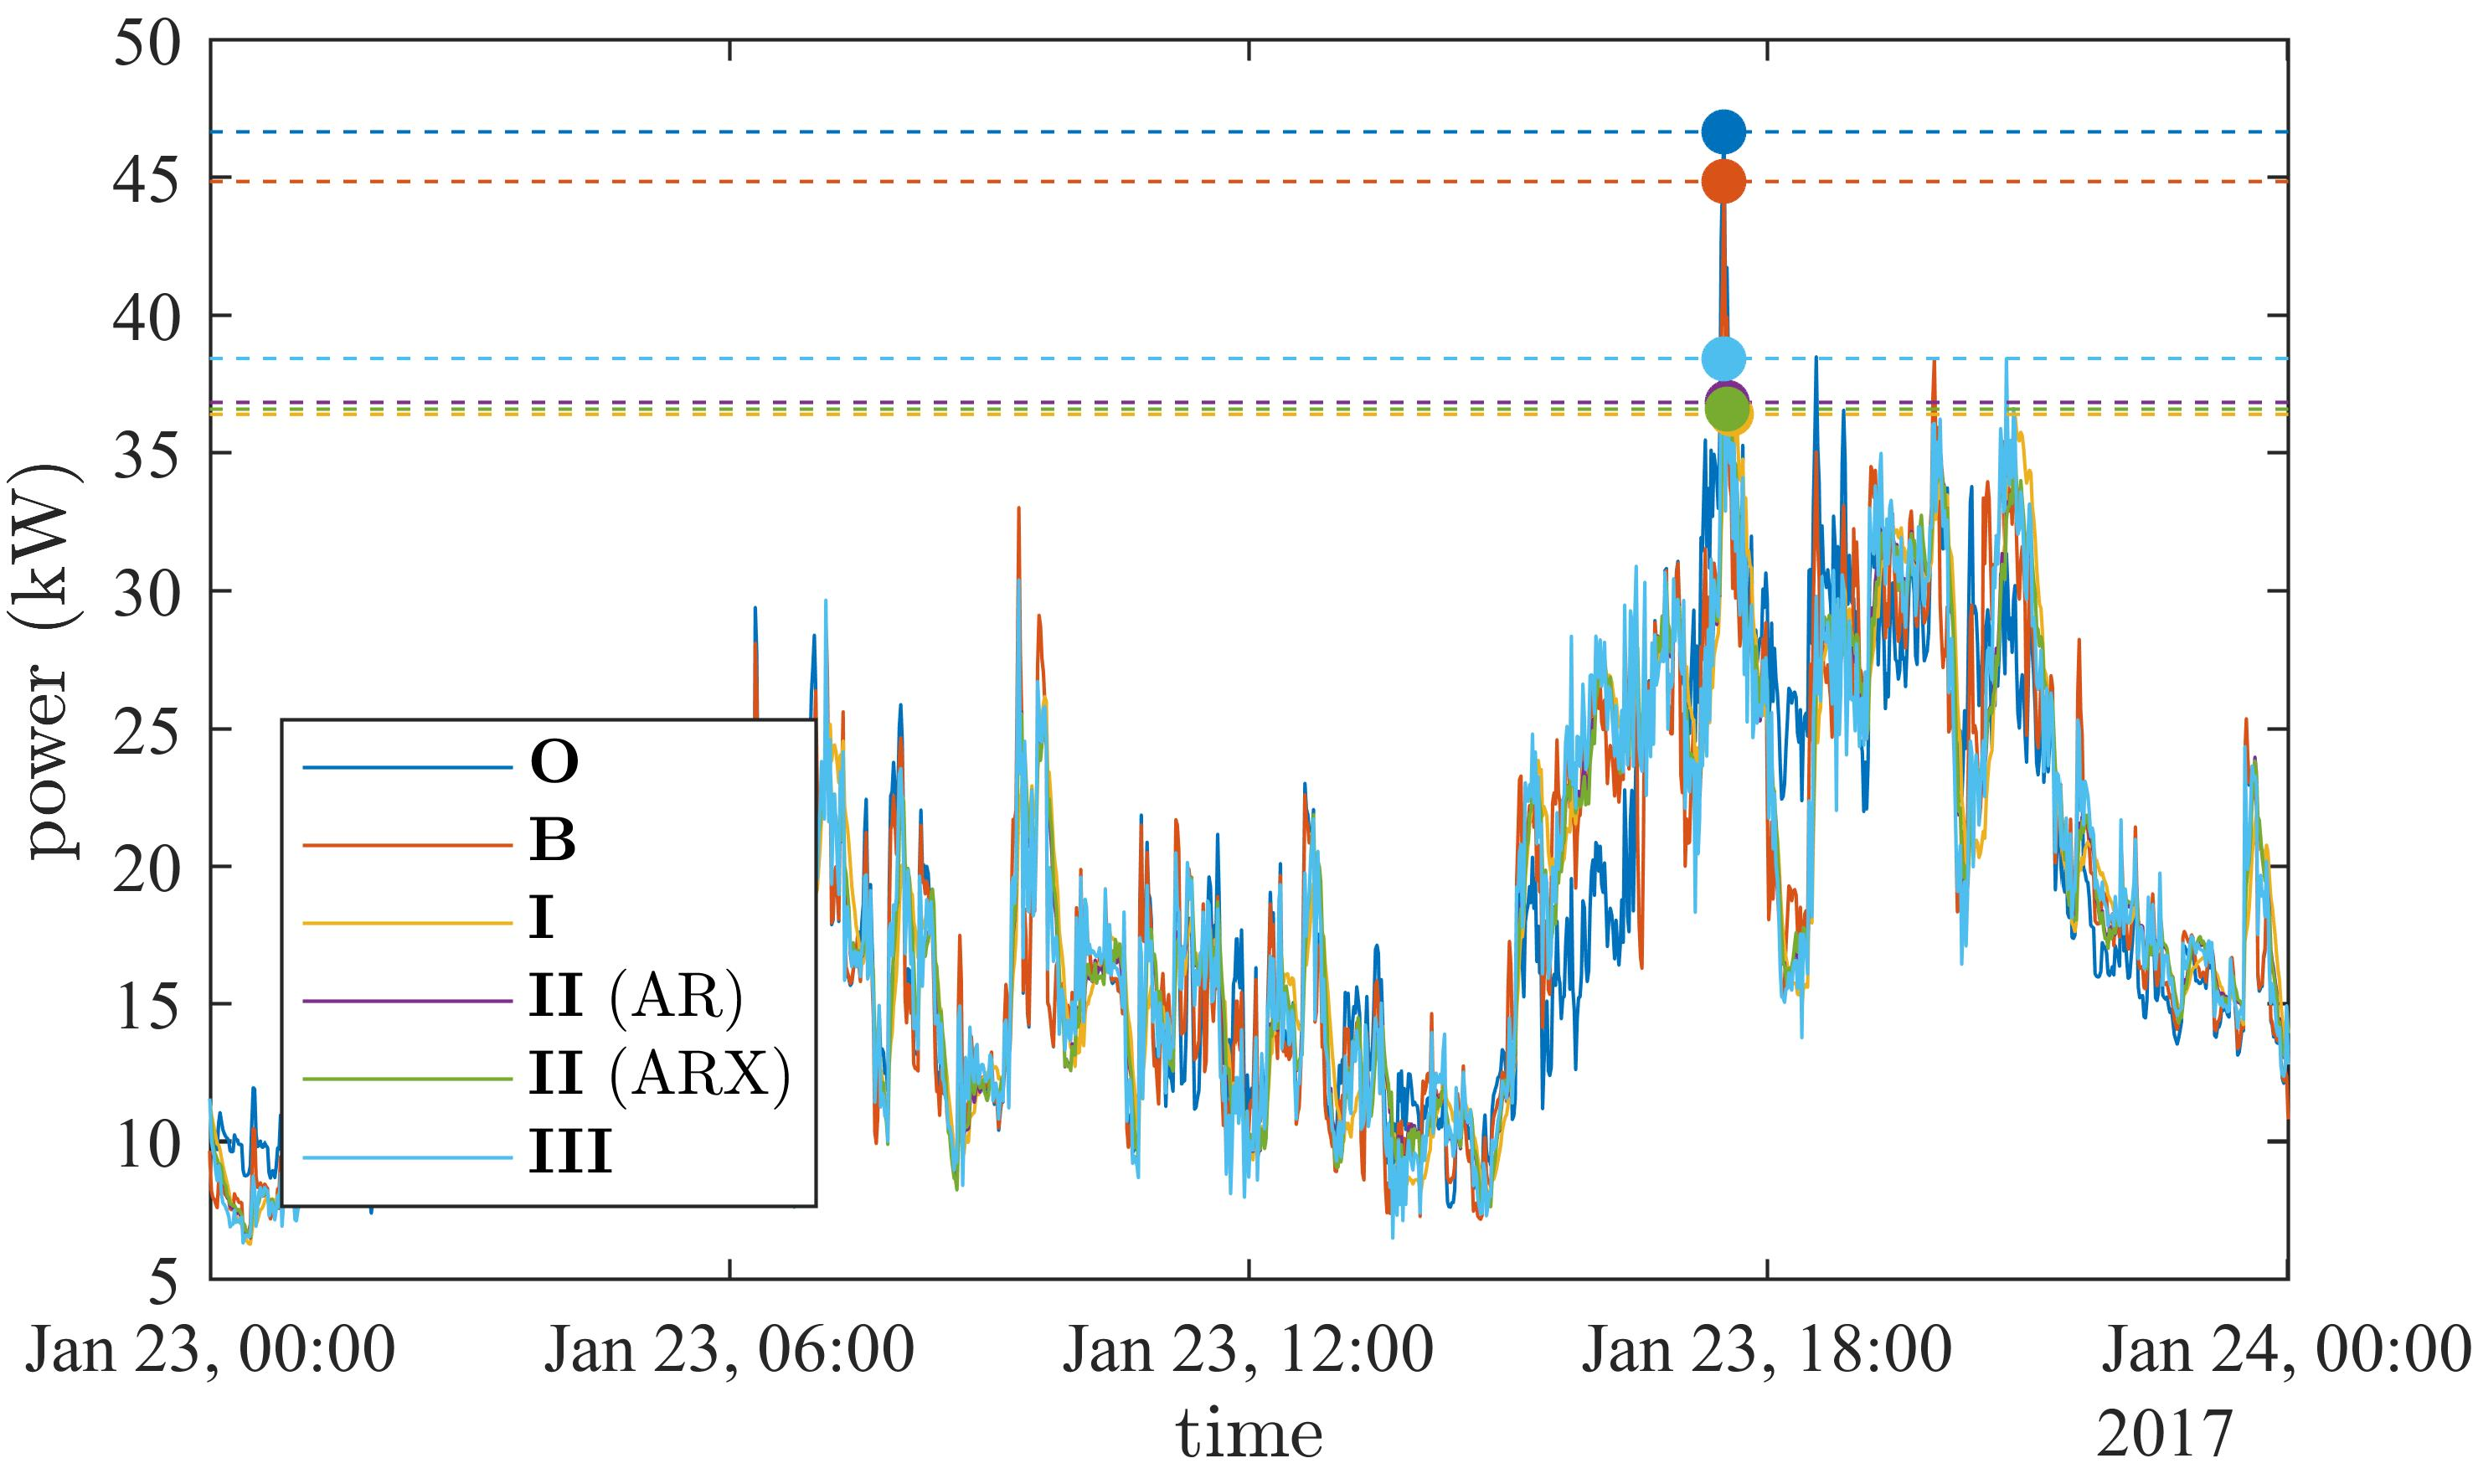
\includegraphics{_chapter2/fig/day-peak-1}
		\label{ch2:subfig:day-peak-total}
	}\\
	\subfloat[]{%
		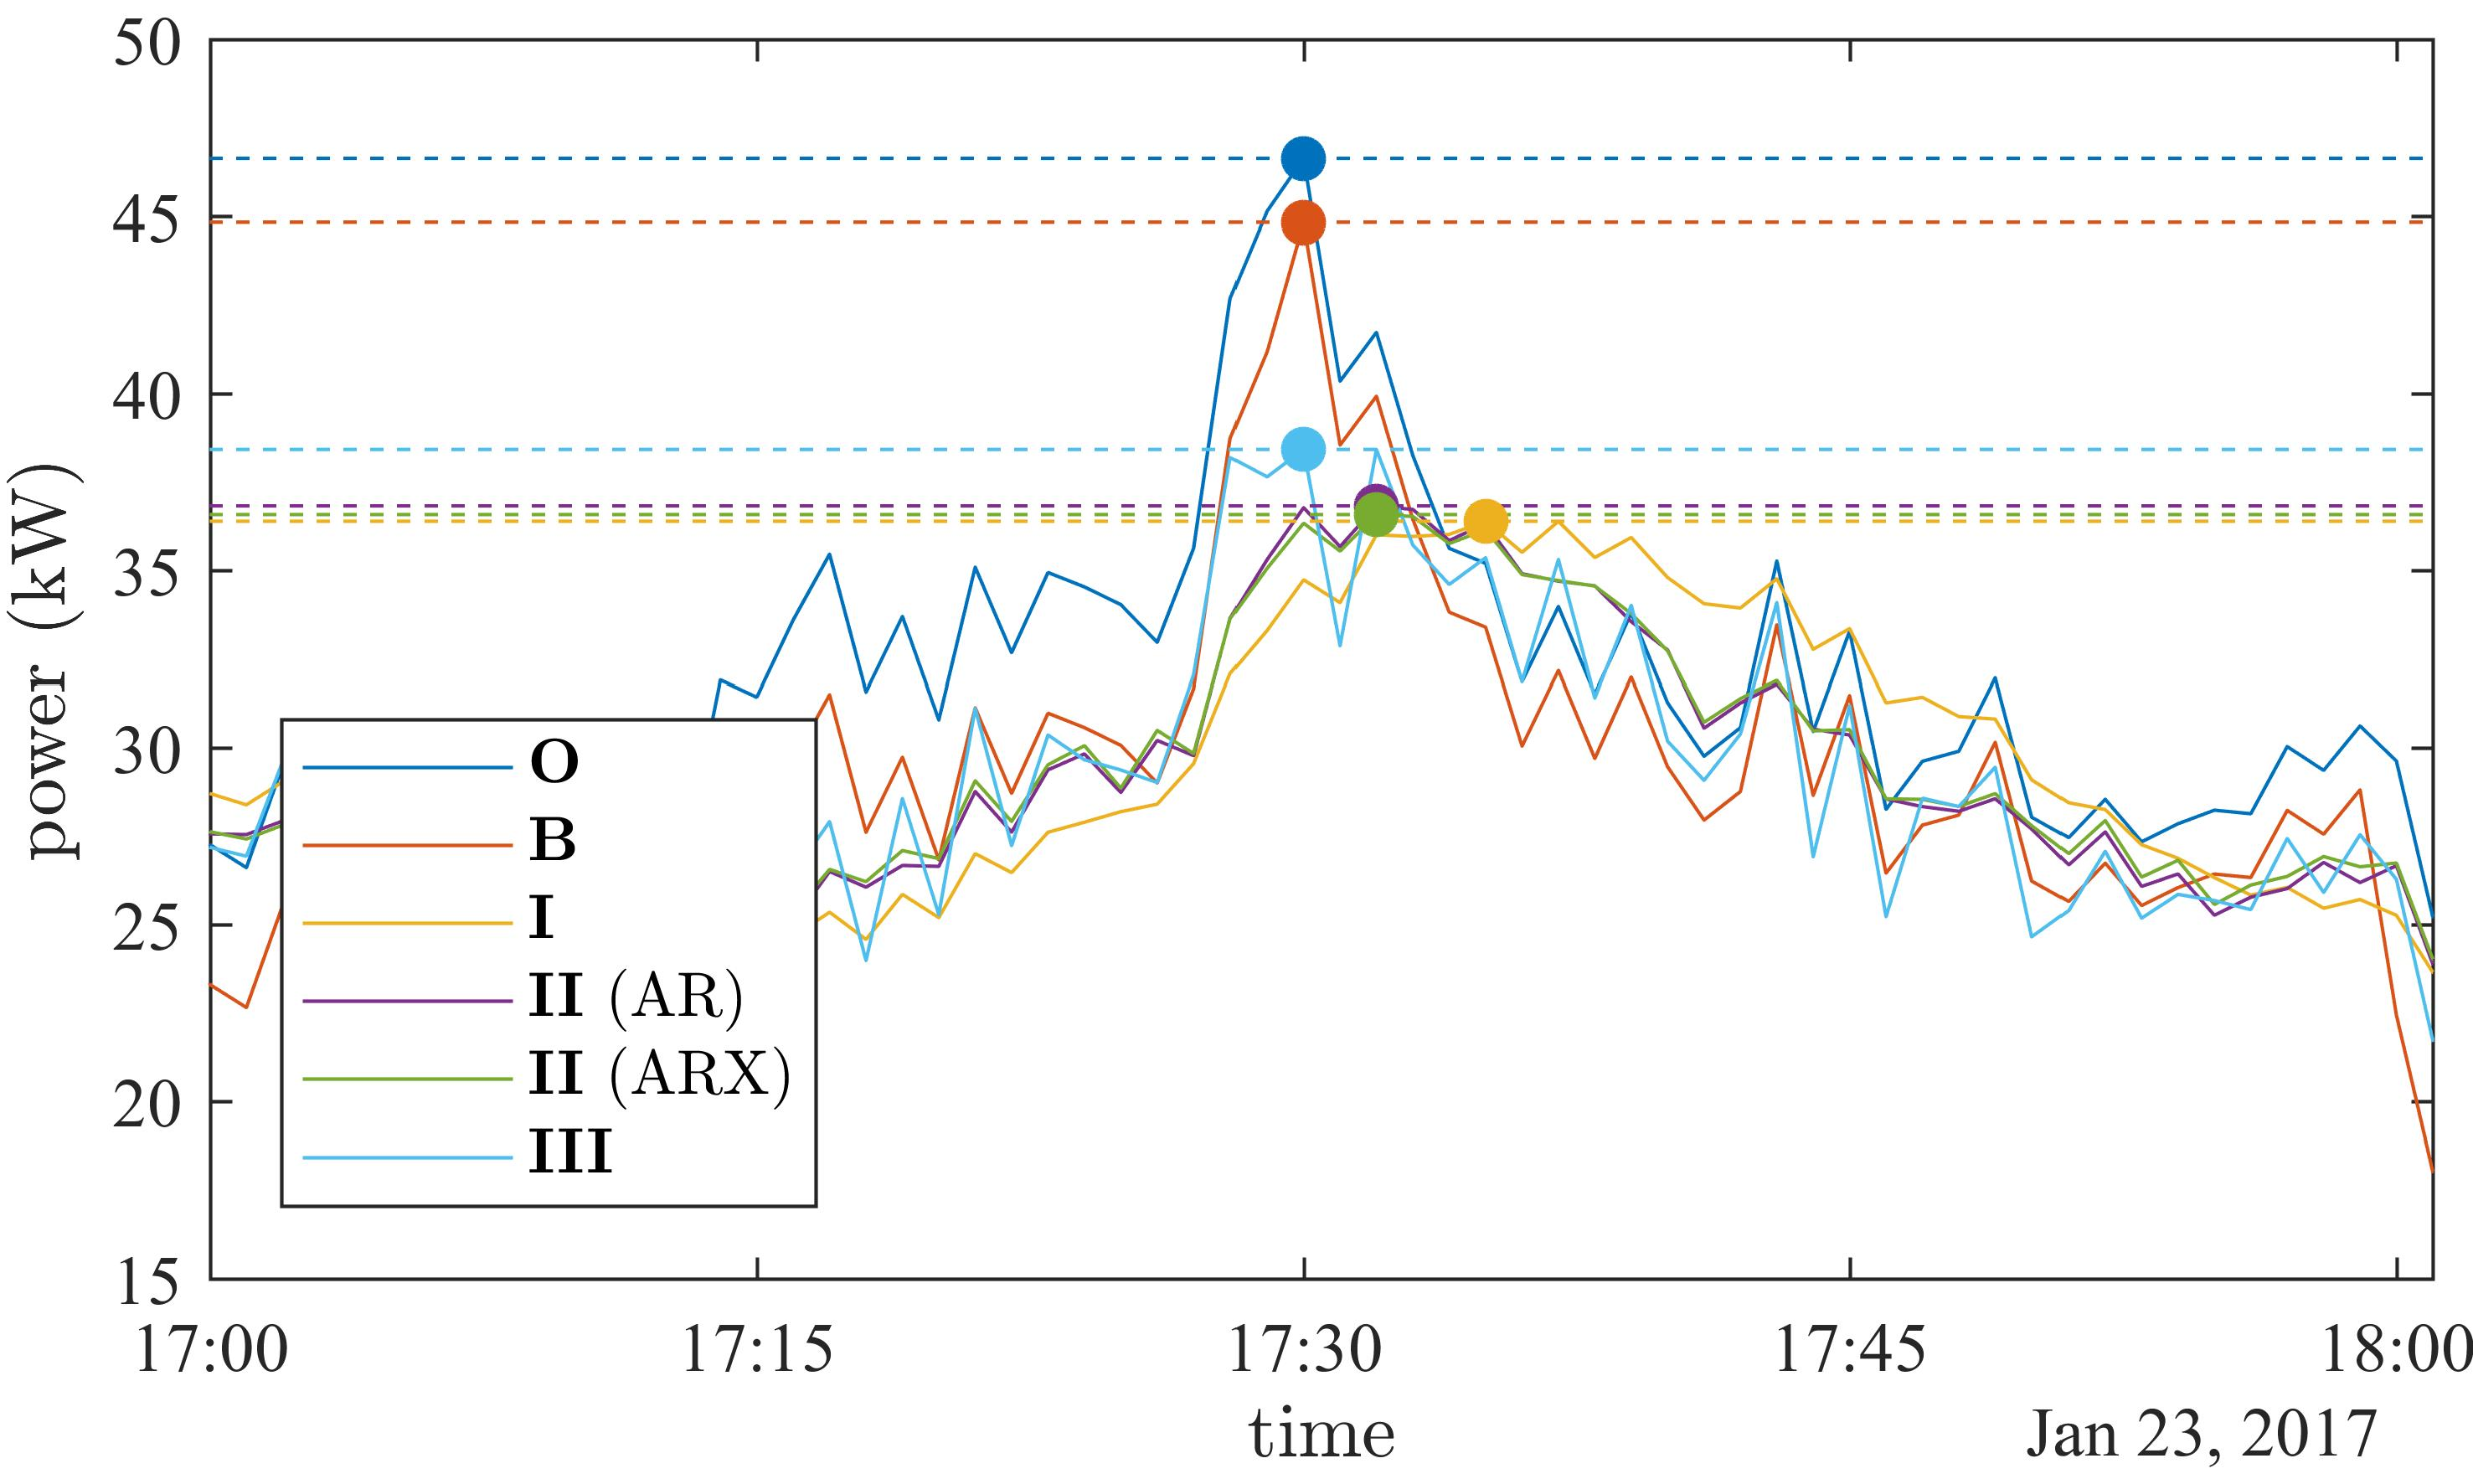
\includegraphics{_chapter2/fig/day-peak-1-zoom}
		\label{ch2:subfig:day-peak-zoomed}
	}
%	\subfloat[]{%
%		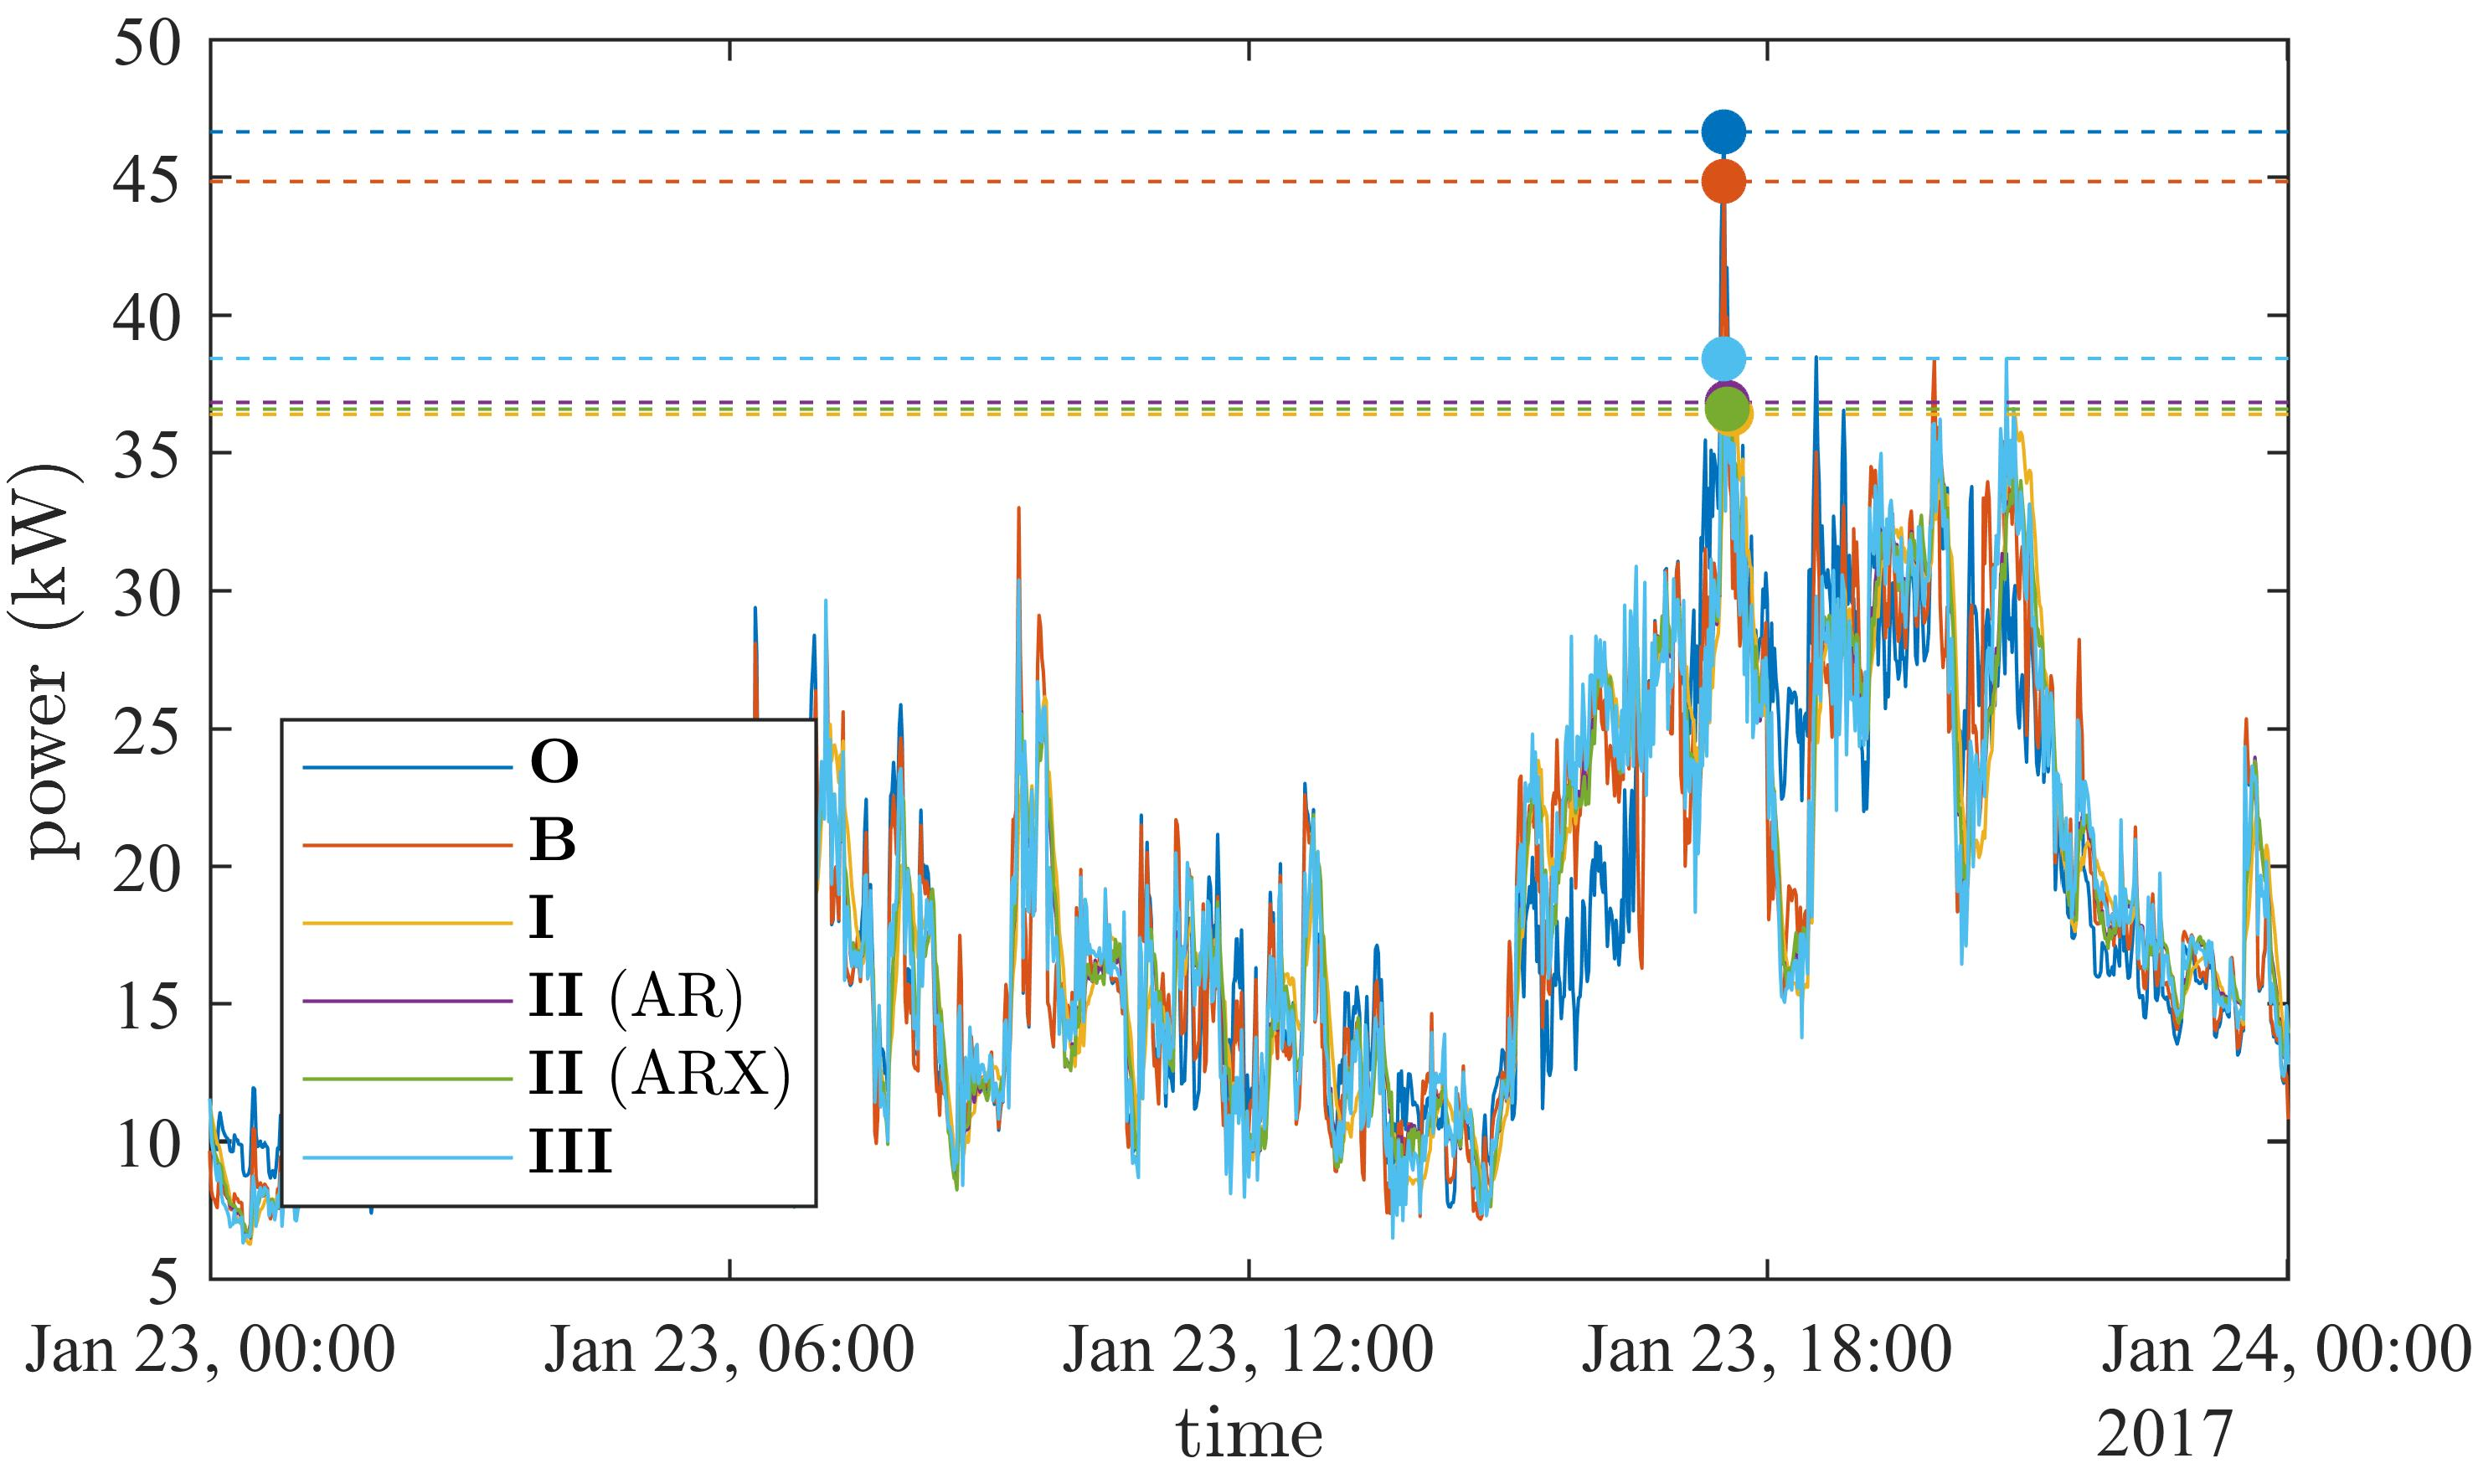
\includegraphics{_chapter2/fig/day-peak-1}
%		\label{ch2:subfig:day-peak-1}
%	}
%	\vspace{0mm}
%	\subfloat[]{%
%		\includegraphics{_chapter2/fig/day-peak-2}
%		\label{ch2:subfig:day-peak-2}
%	}
	\caption{Time series performance over a single day when using realistic load forecasts (total day in Figure \ref{ch2:subfig:day-peak-total}, and zoomed in on critical period in Figure \ref{ch2:subfig:day-peak-zoomed}).}
	\label{ch2:fig:day-peak}
\end{figure}

A single day was plotted in Figure \ref{ch2:fig:day-peak}, which shows the time-series improvements, yielded by the ESMU operation.
For visual clarity, Figure \ref{ch2:subfig:day-peak-total} and \ref{ch2:subfig:day-peak-zoomed} show, respectively, the entire day and a zoomed in version of the ESMU impact.
It can be observed, that the unmodified demand profile, i.e. the original case (case \textbf{O}), and the case where scheduled half-hourly ESMU operation is applied, i.e. the  baseline case (\textbf{B}), result in noticeably higher load peaks than any of the three adjustment cases.
More specifically, the original peak reduction (which is equal to the scheduled ESMU power) was 1.8kW (3.9\% reduction), whereas the average peak reduction when adjusting ESMU operation was 9.6kW (20.6\% reduction).
Furthermore, figure \ref{ch2:subfig:day-peak-total} highlights the volatility of the underlying data, which was not included in the half-hourly ESMU schedule.

Interestingly, both the standard AR and the exogenous AR estimation models, that were used in case \textbf{II}, performed very similar and show little to no significant difference in peak reduction performance.
Equally noteworthy is the fact, that the simplest prediction methods of them all, i.e. the method of ``assuming a power repetition occurs'', like in case \textbf{I}, yields good results, too.
The amount by which the three cases were able to reduce the daily peak load is also highlighted with the corresponding horizontal dashed lines and dots located at the point of peak load.
These initial findings show that every single version of dynamic control reduces peak load further, when compared to the baseline case \textbf{O}.
This finding is as tabulated in Table \ref{ch2:tab:ts-table}, and suggest that the prediction mechanism by itself did play a small role in compensating for demand volatility.

\begin{table}\centering
%	\begin{tabular}{r | c}
%		case & peak load\\% & ideal forecast\\
%		\hline
%		\textbf{O} & 46.6kW\\
%		\textbf{B} & 44.8kW\\
%		\textbf{I} & 36.4kW\\% & \textbf{IV}\\
%		\textbf{II} (AR) & 36.8kW\\% & \textbf{V}\\
%		\textbf{II} (ARX) & 36.6kW\\% & \textbf{V}\\
%		\textbf{III} & 38.4kW\\% & \textbf{VI}\\
%	\end{tabular}
	\begin{tabular}{r | c | c | c | c | c | c}
		\multirow{2}{*}{case} & \multirow{2}{*}{\textbf{O}} & \multirow{2}{*}{\textbf{B}} & \multirow{2}{*}{\textbf{I}} & \textbf{II} & \textbf{II} & \multirow{2}{*}{\textbf{III}}\\% & ideal forecast\\
		& & & & \tiny{(AR)} & \tiny{(ARX)} & \\% & ideal forecast\\
		\hline
		peak & \multirow{2}{*}{46.6} & \multirow{2}{*}{44.8} & \multirow{2}{*}{36.4} & \multirow{2}{*}{36.8} & \multirow{2}{*}{36.6} & \multirow{2}{*}{38.4}\\
		(kW) & & & & & & \\
	\end{tabular}
	\caption{Peak reduction in time-series sample}
	\label{ch2:tab:ts-table}	
\end{table}

However, the general magnitude of peak reduction performance can only be assessed if the complete dataset is evaluated.
Hence, the next section compares the daily peak load reduction from the application of each case.

\subsection{Daily peak reduction}

\begin{figure}\centering
	\subfloat[]{%
		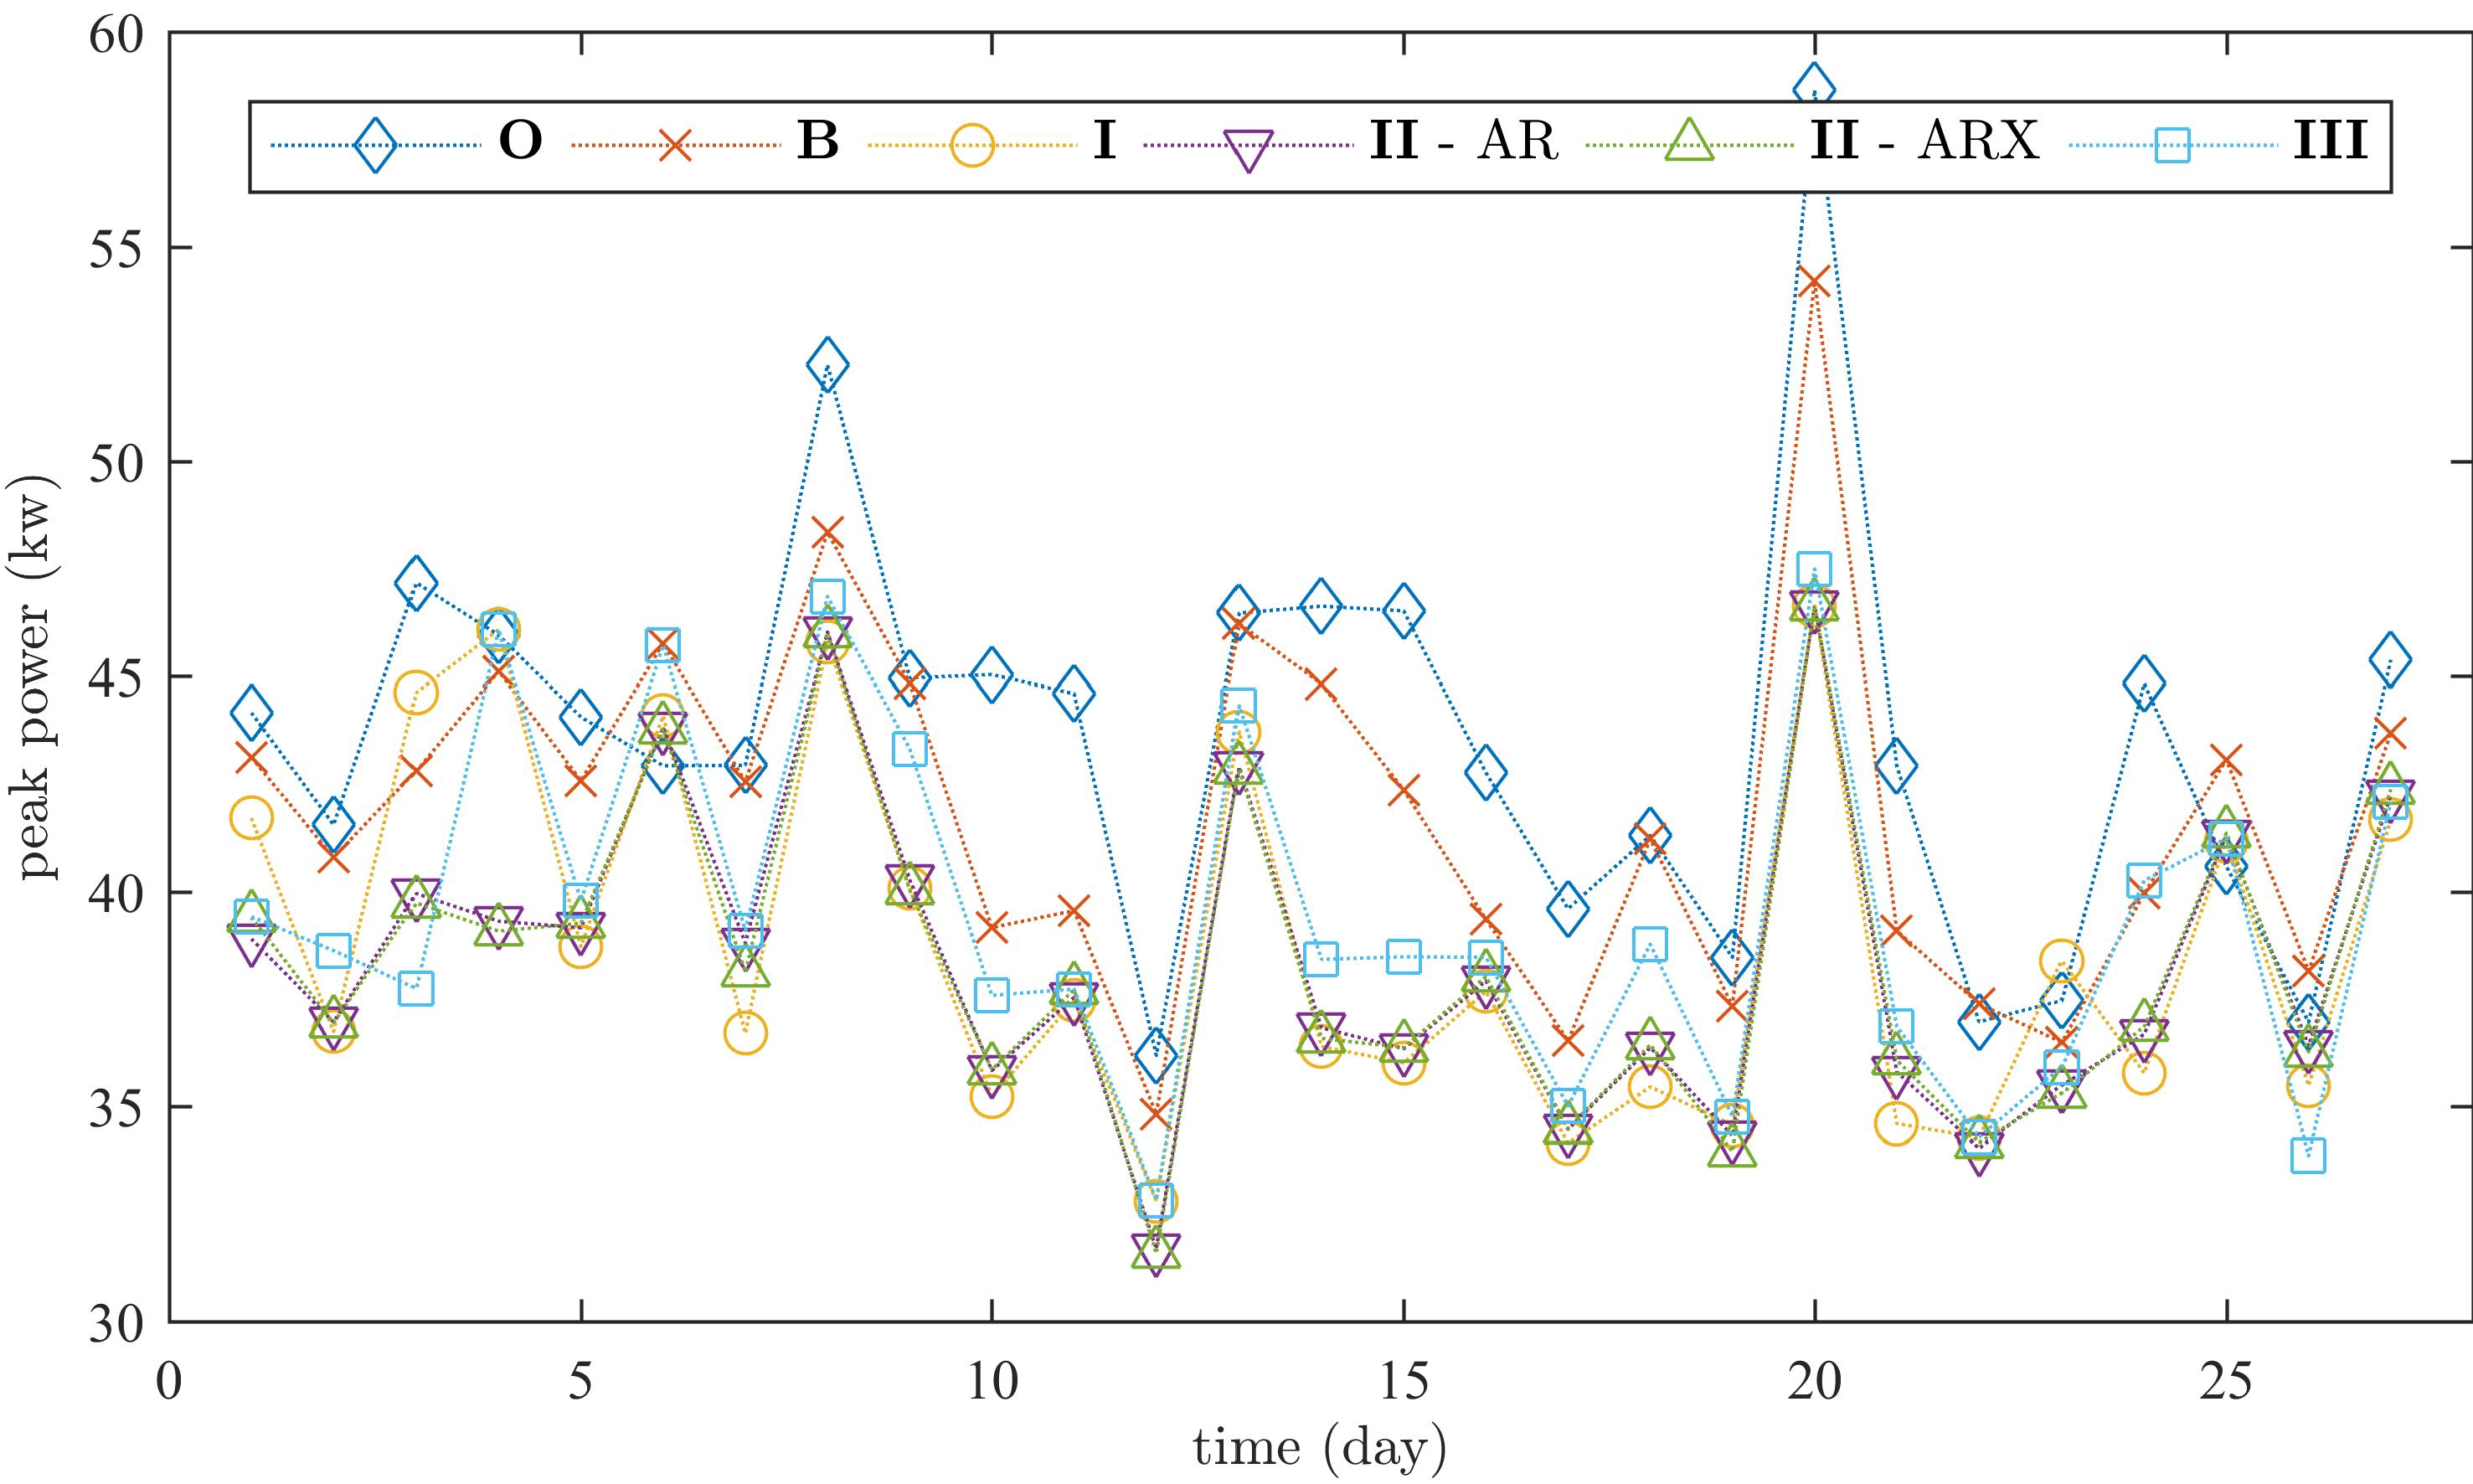
\includegraphics{_chapter2/fig/daily-peaks-1}
		\label{ch2:subfig:daily-peaks}
	}\\
	\subfloat[]{%
		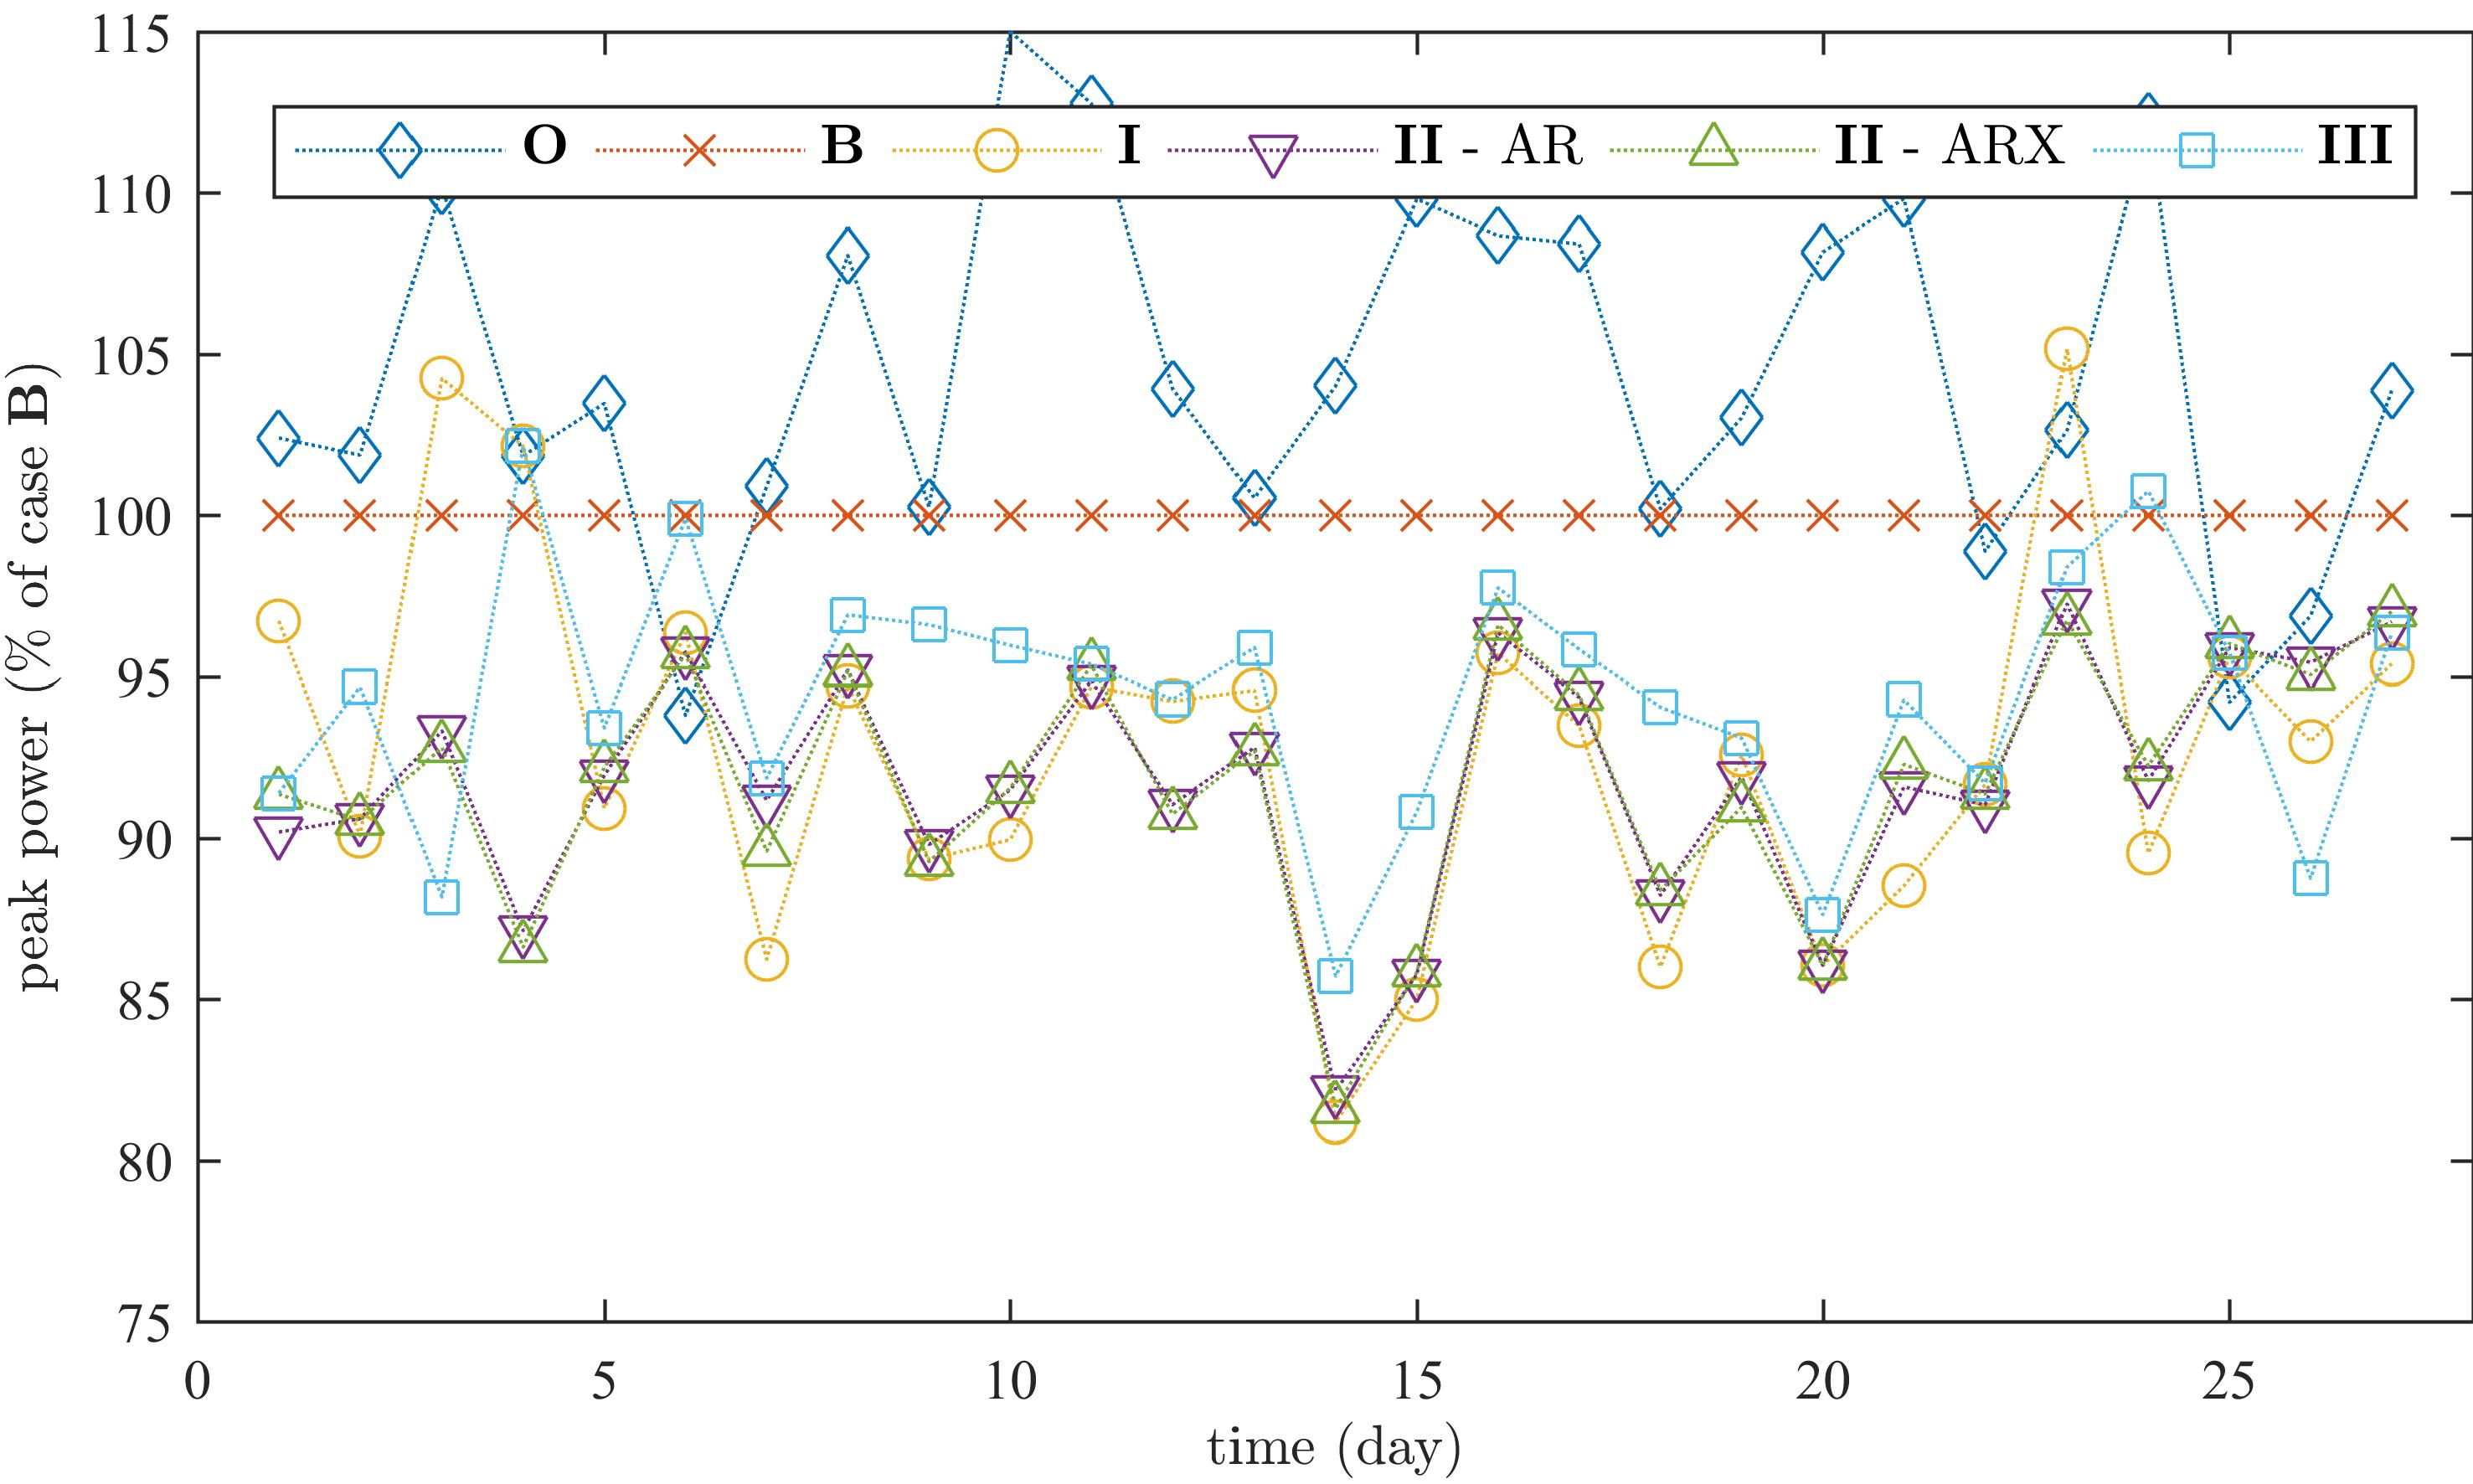
\includegraphics{_chapter2/fig/daily-peaks-1-percentage}
		\label{ch2:subfig:daily-peaks-percentage}
	}
	\caption{Daily peak reduction when using realistic forecasts as: (\ref{ch2:subfig:daily-peaks}) peak power values; (\ref{ch2:subfig:daily-peaks-percentage}) percentage of original case \textbf{B}.}
	\label{ch2:fig:daily-peaks}
\end{figure}

In Figure \ref{ch2:fig:daily-peaks}, every day's power peak was extracted, similar to the procedure used for Figure \ref{ch2:fig:day-peak}.
Here, however, both the actual power peaks as well as the relative power improvements, i.e. in comparison to the original power peak, were plotted.
This was done in Figure \ref{ch2:subfig:daily-peaks} and Figure \ref{ch2:subfig:daily-peaks-percentage}, respectively.
From both plots, it can be seen that controlling ESMU using the proposed dynamic control lowers peak load, especially when the underlying ESMU schedule originally worsened and increased peak load.
Such behaviour can be observed for e.g. days six, where the half-hourly ESMU schedule worsened the actual load peak, yet ESMU schedule adjustment mechanisms compensated for this error.
Nonetheless, having a larger set of peak reduction results to compare the dynamic control's performance against the baseline cases, sensitivity to the underlying power prediction approaches become apparent, too.
For example, case \textbf{I}, using the simplest prediction mechanism, underperformed on day 23 and worsened the peak power.
In order to get a better idea of the general peak reduction performance when applying case \textbf{I}, \textbf{II} or \textbf{III}, the Probability Density Function was estimated and plotted in the following section.

\subsection{Probability of peak reduction}
\label{ch2:subsec:probability-of-peak-reduction}

\begin{figure}\centering
	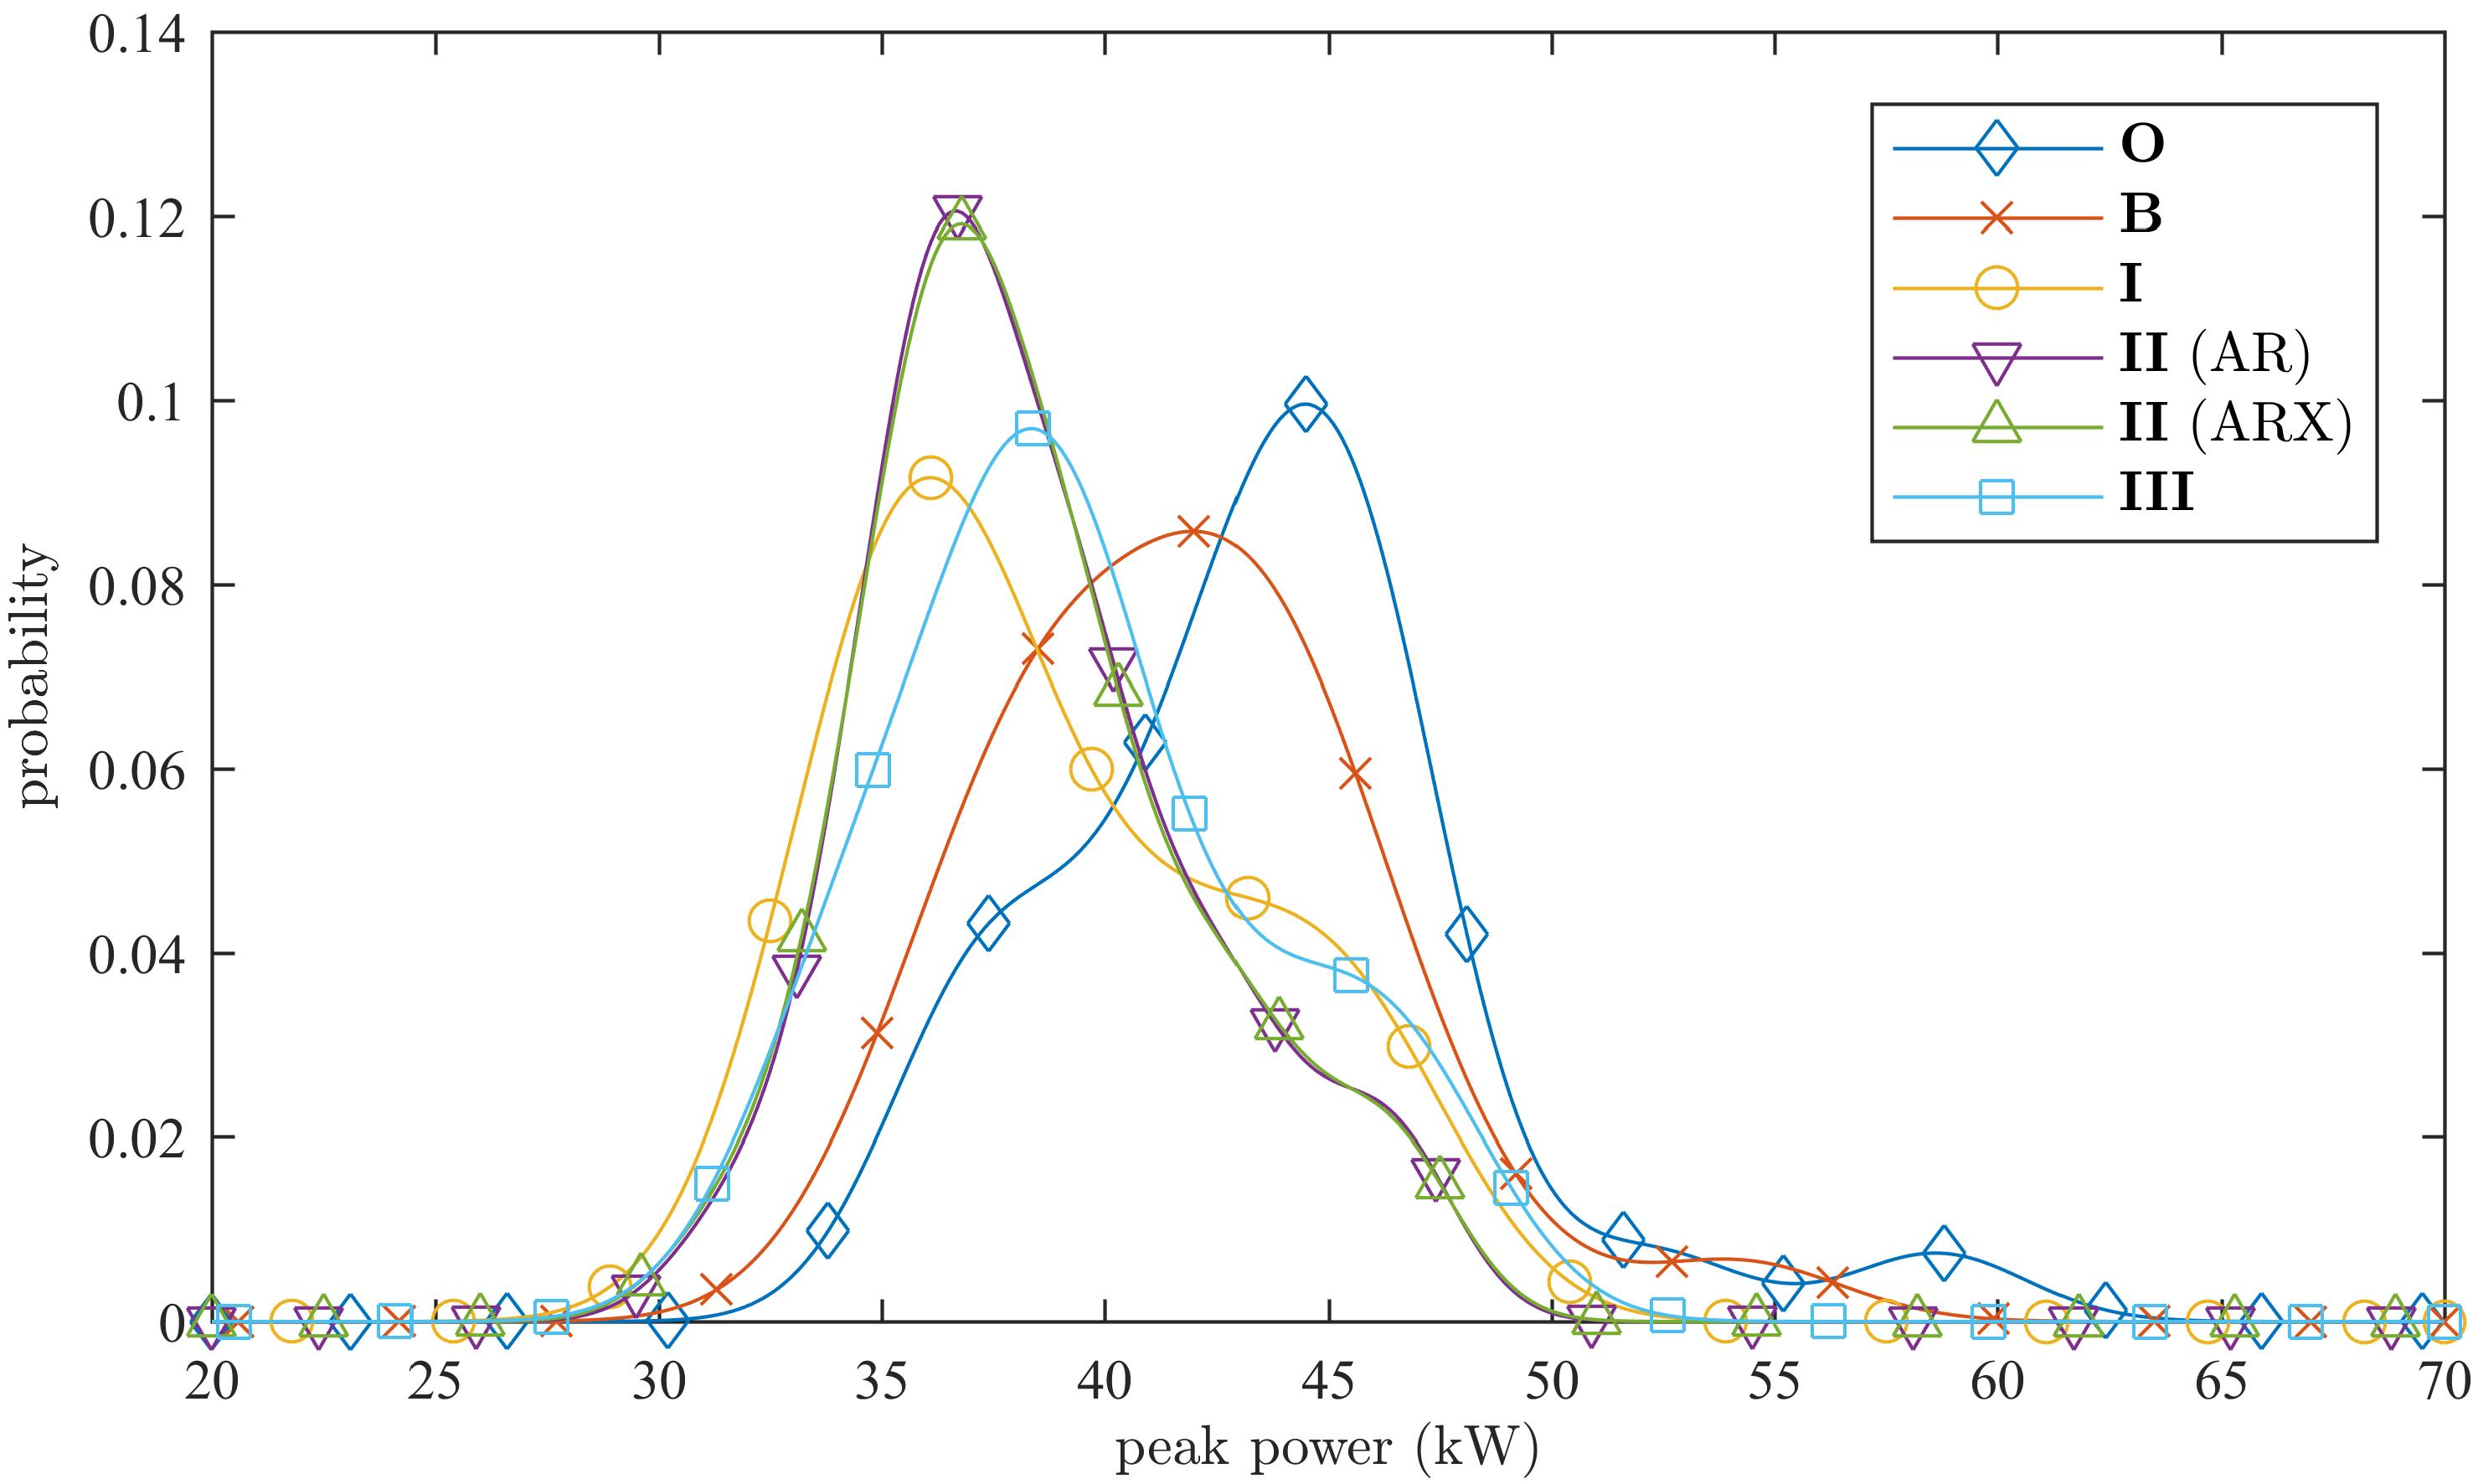
\includegraphics{_chapter2/fig/pdf-1-avg}
%	\subfloat[]{%
%		\includegraphics{_chapter2/fig/pdf-1}
%		\label{ch2:subfig:peak-pdf-1}
%	}
%	\vspace{0mm}
%	\subfloat[]{%
%		\includegraphics{_chapter2/fig/pdf-2}
%		\label{ch2:subfig:peak-pdf-2}
%	}
	\caption{Probability of load peak when using realistic forecasts.}
	\label{ch2:fig:peak-pdf}
\end{figure}

Using standard kernel density estimation, the PDF was plotted in Figure \ref{ch2:fig:peak-pdf}.
The data used to generate these plots is the same data shown in Figure \ref{ch2:fig:daily-peaks}.
Now, the probability of a peak power occurring is linked to the magnitude of this peak.
It can be seen that case \textbf{O} has the highest probability around a load peak of 45kW, whilst case \textbf{B} has its highest probability around a load peak of 42kW.
This indicates that even the pure half-hourly ESMU schedule had a positive impact on reducing load peaks.
When adjusting the schedule based with the use of the proposed dynamic control, this peak was lowered further.

\begin{figure}\centering
	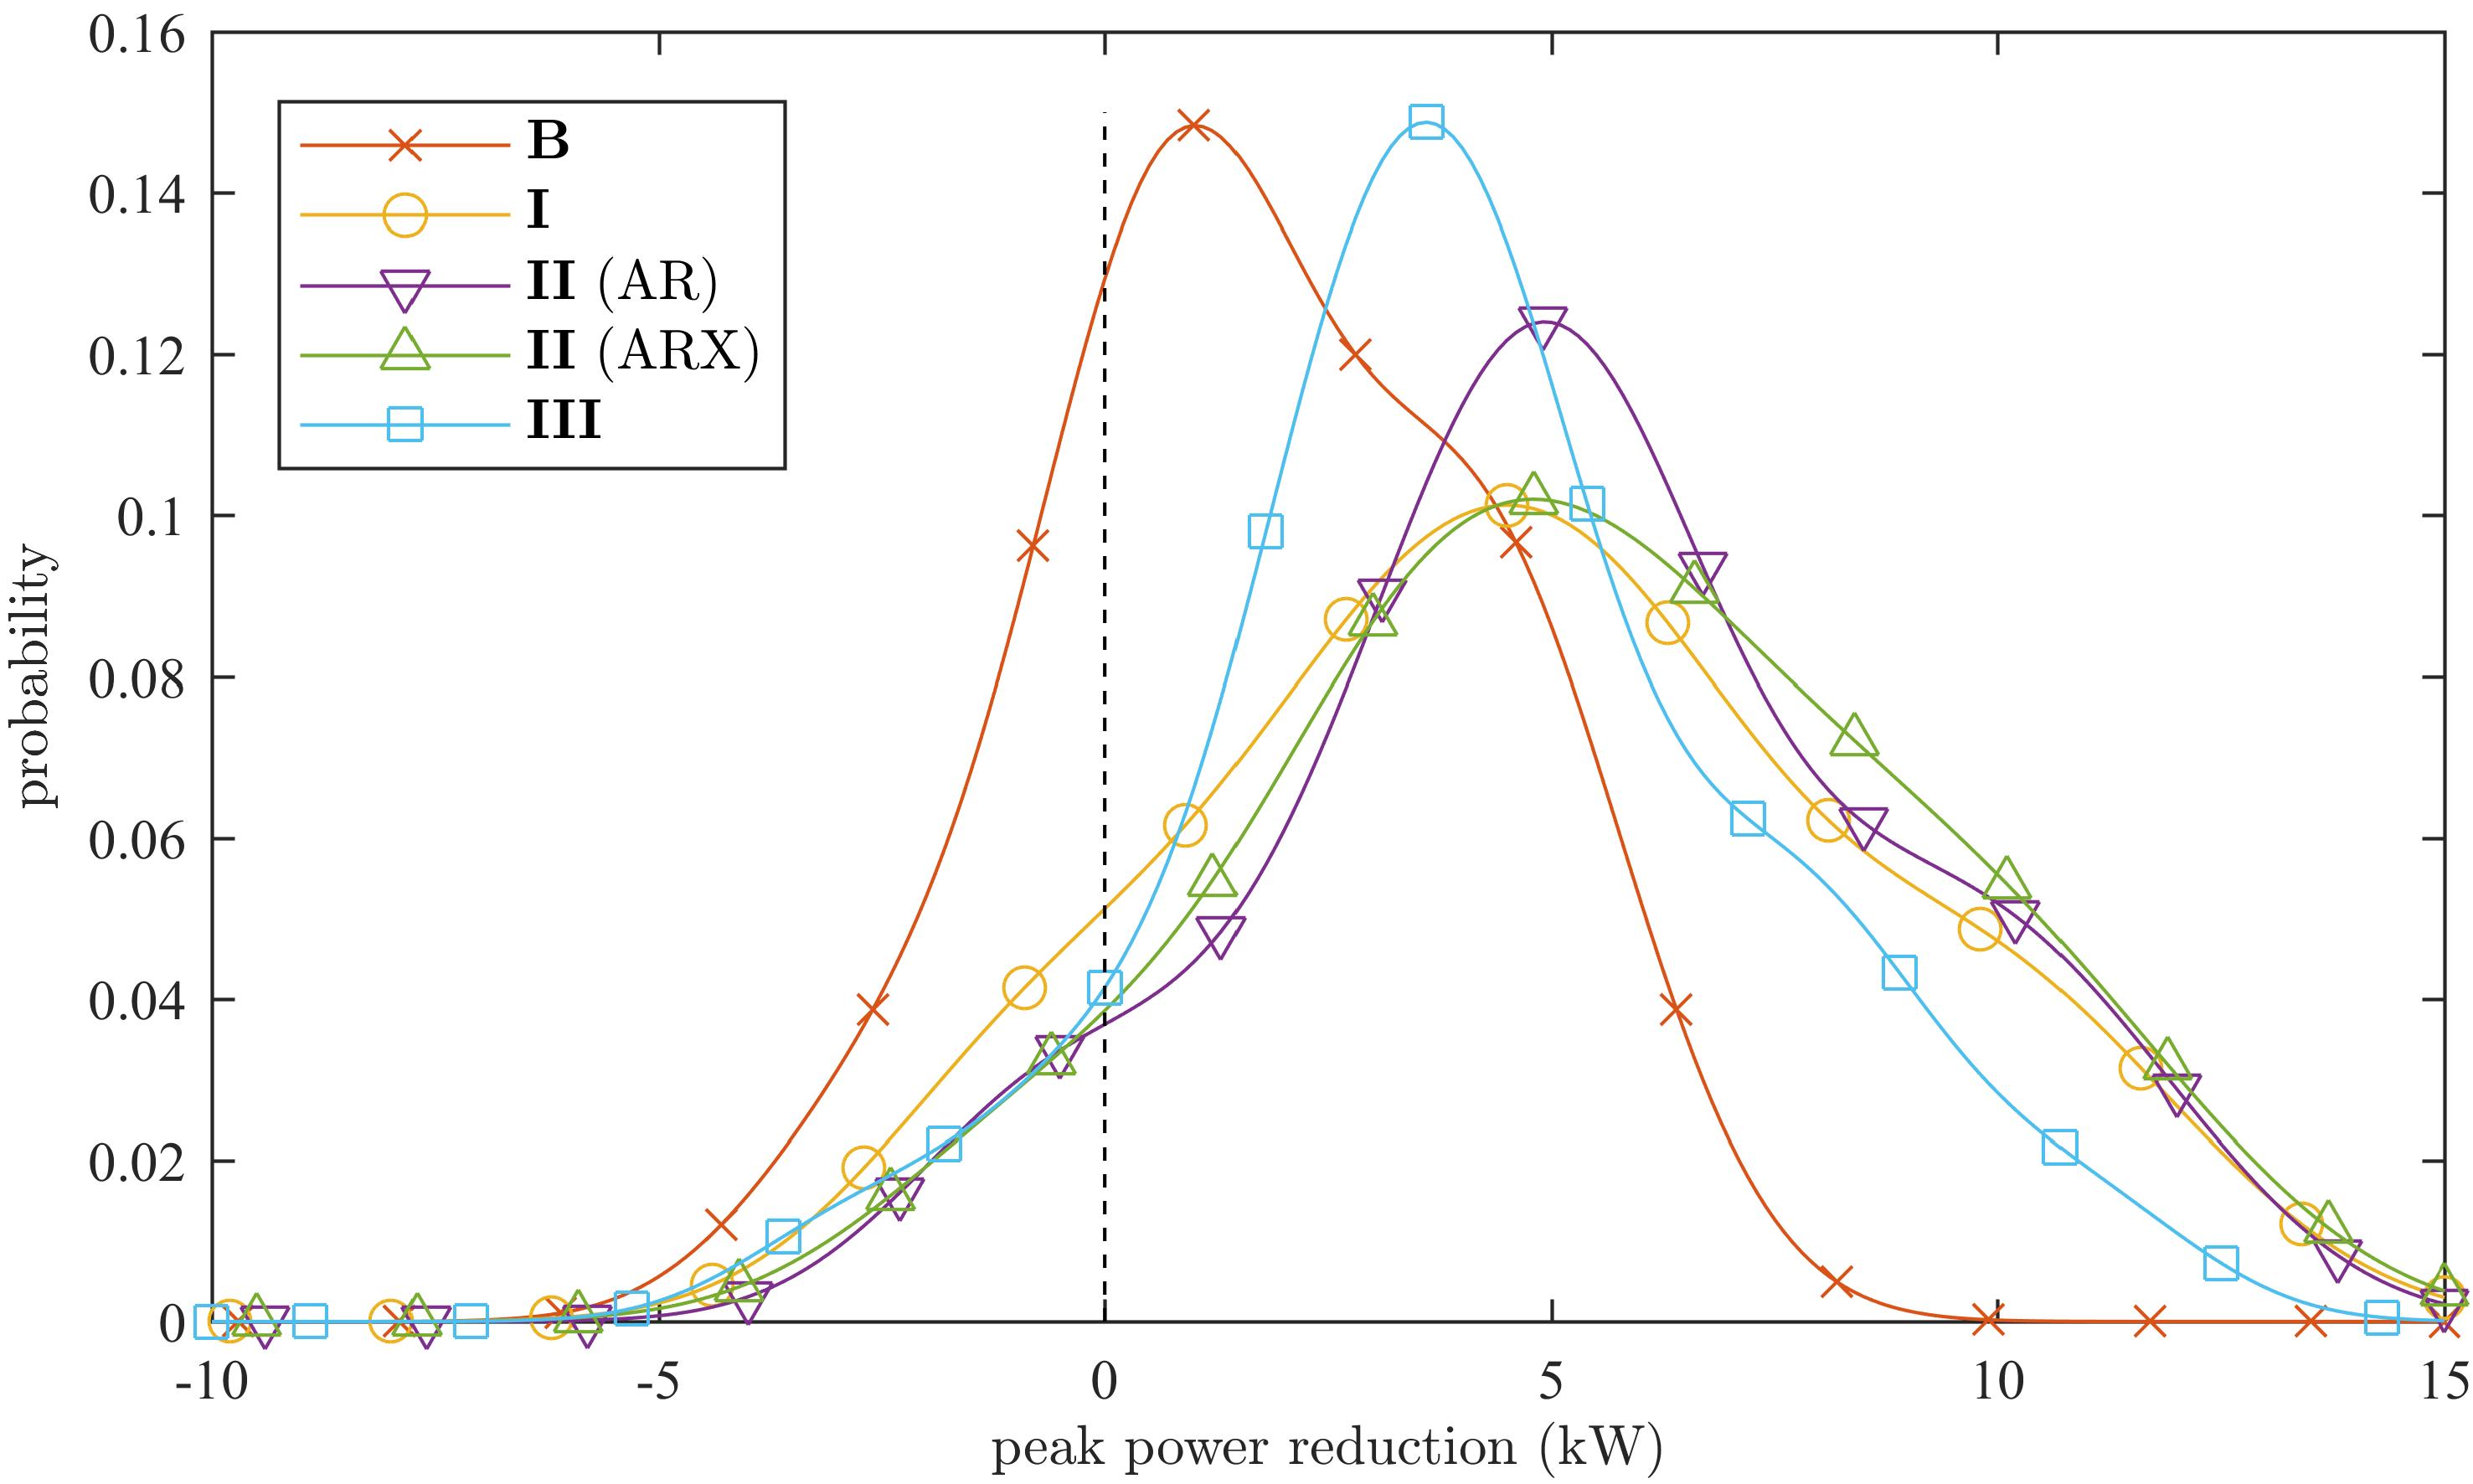
\includegraphics{_chapter2/fig/difference-pdf-1-avg}
%	\subfloat[]{%
%		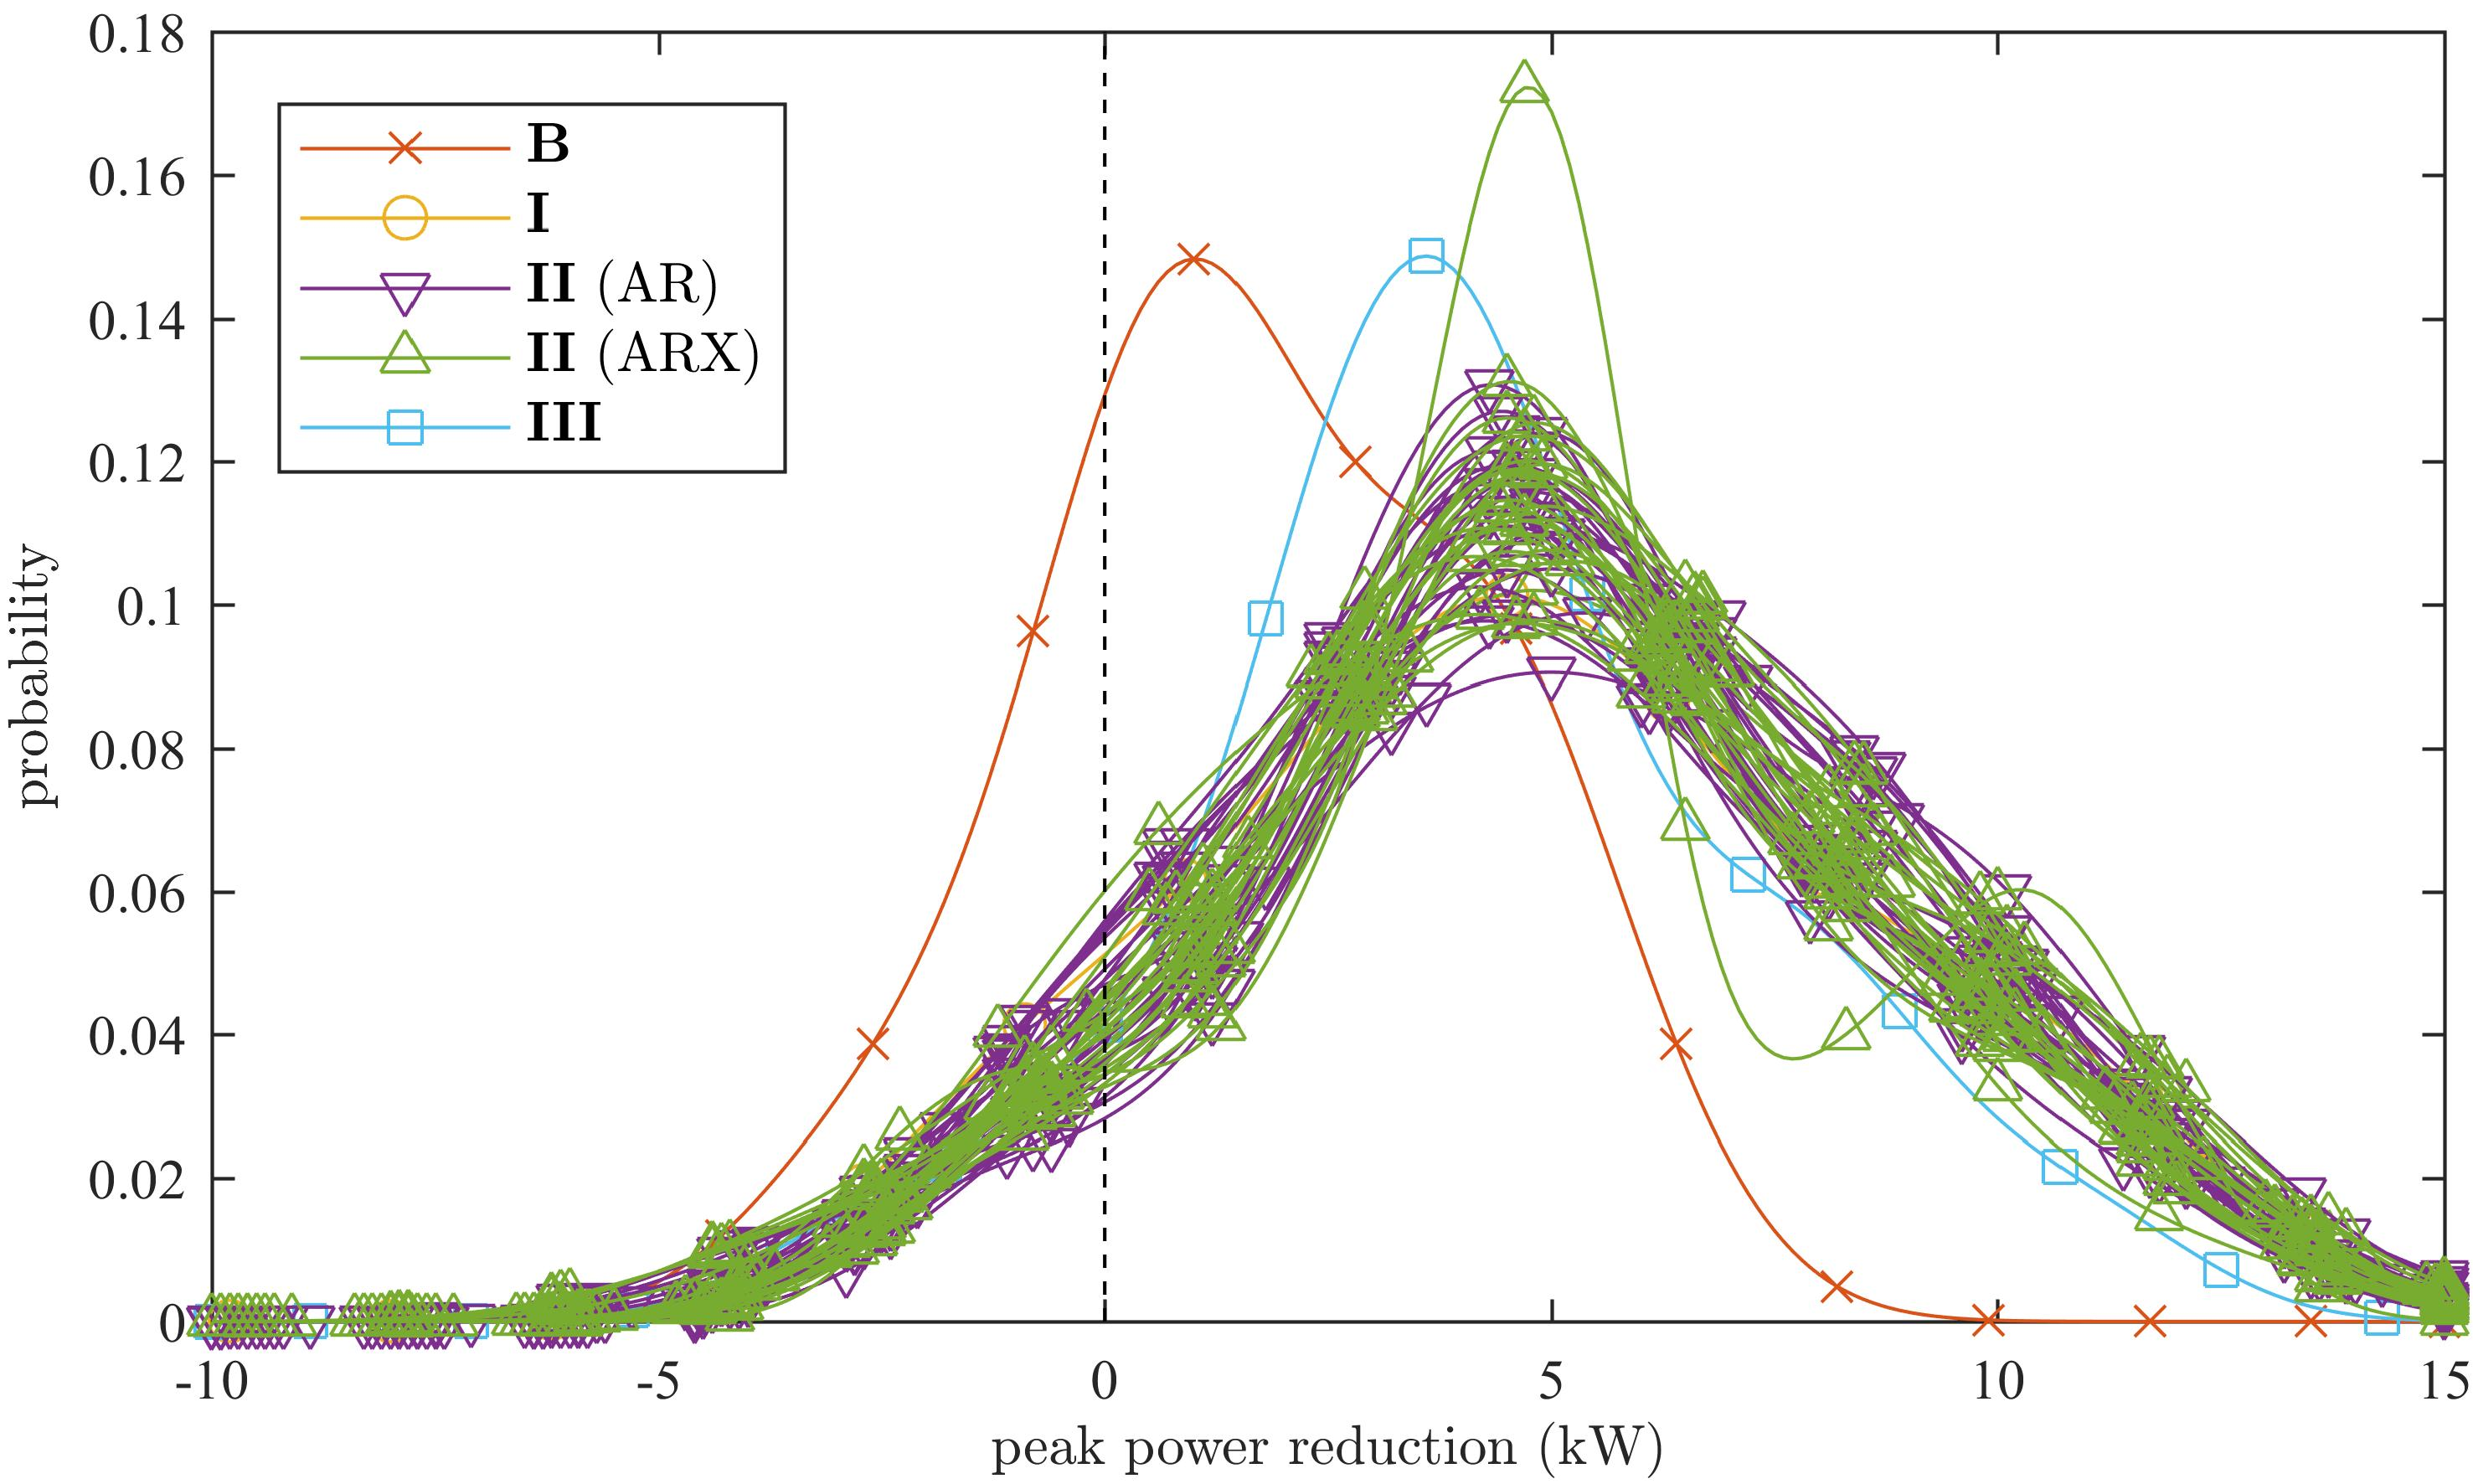
\includegraphics{_chapter2/fig/difference-pdf-1}
%		\label{ch2:subfig:peak-diff-pdf-1}
%	}
%	\vspace{0mm}
%	\subfloat[]{%
%		\includegraphics{_chapter2/fig/difference-pdf-2}
%		\label{ch2:subfig:peak-diff-pdf-2}
%	}
	\caption{Probability of load peak reduction when using realistic forecasts.}
	\label{ch2:fig:peak-diff-pdf}
\end{figure}

Figure \ref{ch2:fig:peak-diff-pdf} takes this analysis even further, where only the difference in peak load to the original case, case \textbf{O}, was plotted.
Now, ESMU impact can easily be seen, since a high probability of positive peak load reduction indicates a beneficial impact of the ESMU operation, whereas a negative peak load reduction (i.e. increased peak load) indicates a worsening performance.
As expected, case \textbf{O} has a slight positive impact on the system, whilst a cumulative probability of more than 25\% (i.e. area under curve of case \textbf{O} to the left of 0kW) suggests that the peak might be worsened one in four times.
Using dynamic control with its simplest prediction method however, i.e. case \textbf{I}, lowered this probability to only 11.8\%, with the AR model in case \textbf{II} performing best at only 8\%.

Beside the reduced probability of missing or worsening peak load, the probability of having a larger positive impact is also increased when using the dynamic control.
Whilst the probability of reducing load peaks by 1.7kW or more was at 50\% for case \textbf{B}, case \textbf{I} increased this probability to 77.7\%, case \textbf{II} to 84.5 5\% (AR) / 83.1\% (ARX), and case \textbf{III} to 79.8\%.
When comparing the three dynamic control cases with each other, Figure \ref{ch2:fig:peak-diff-pdf} indicates that case \textbf{II} using an AR model for MPC performed best at reducing peak loads.

\subsection{Impact of varying the model's length}

The subsequent results are intended to reveal whether the length of the AR/ARX model impacted the peak reduction performance.
To do so, the same procedure was use as shown in Section \ref{ch2:subsec:probability-of-peak-reduction}, but the length of the AR and ARX models was varied from five minutes to two hours.
Therefore, the MPC of the dynamic control took into account a longer power history to potentially improve the prediction of the next power.

\begin{figure}\centering
	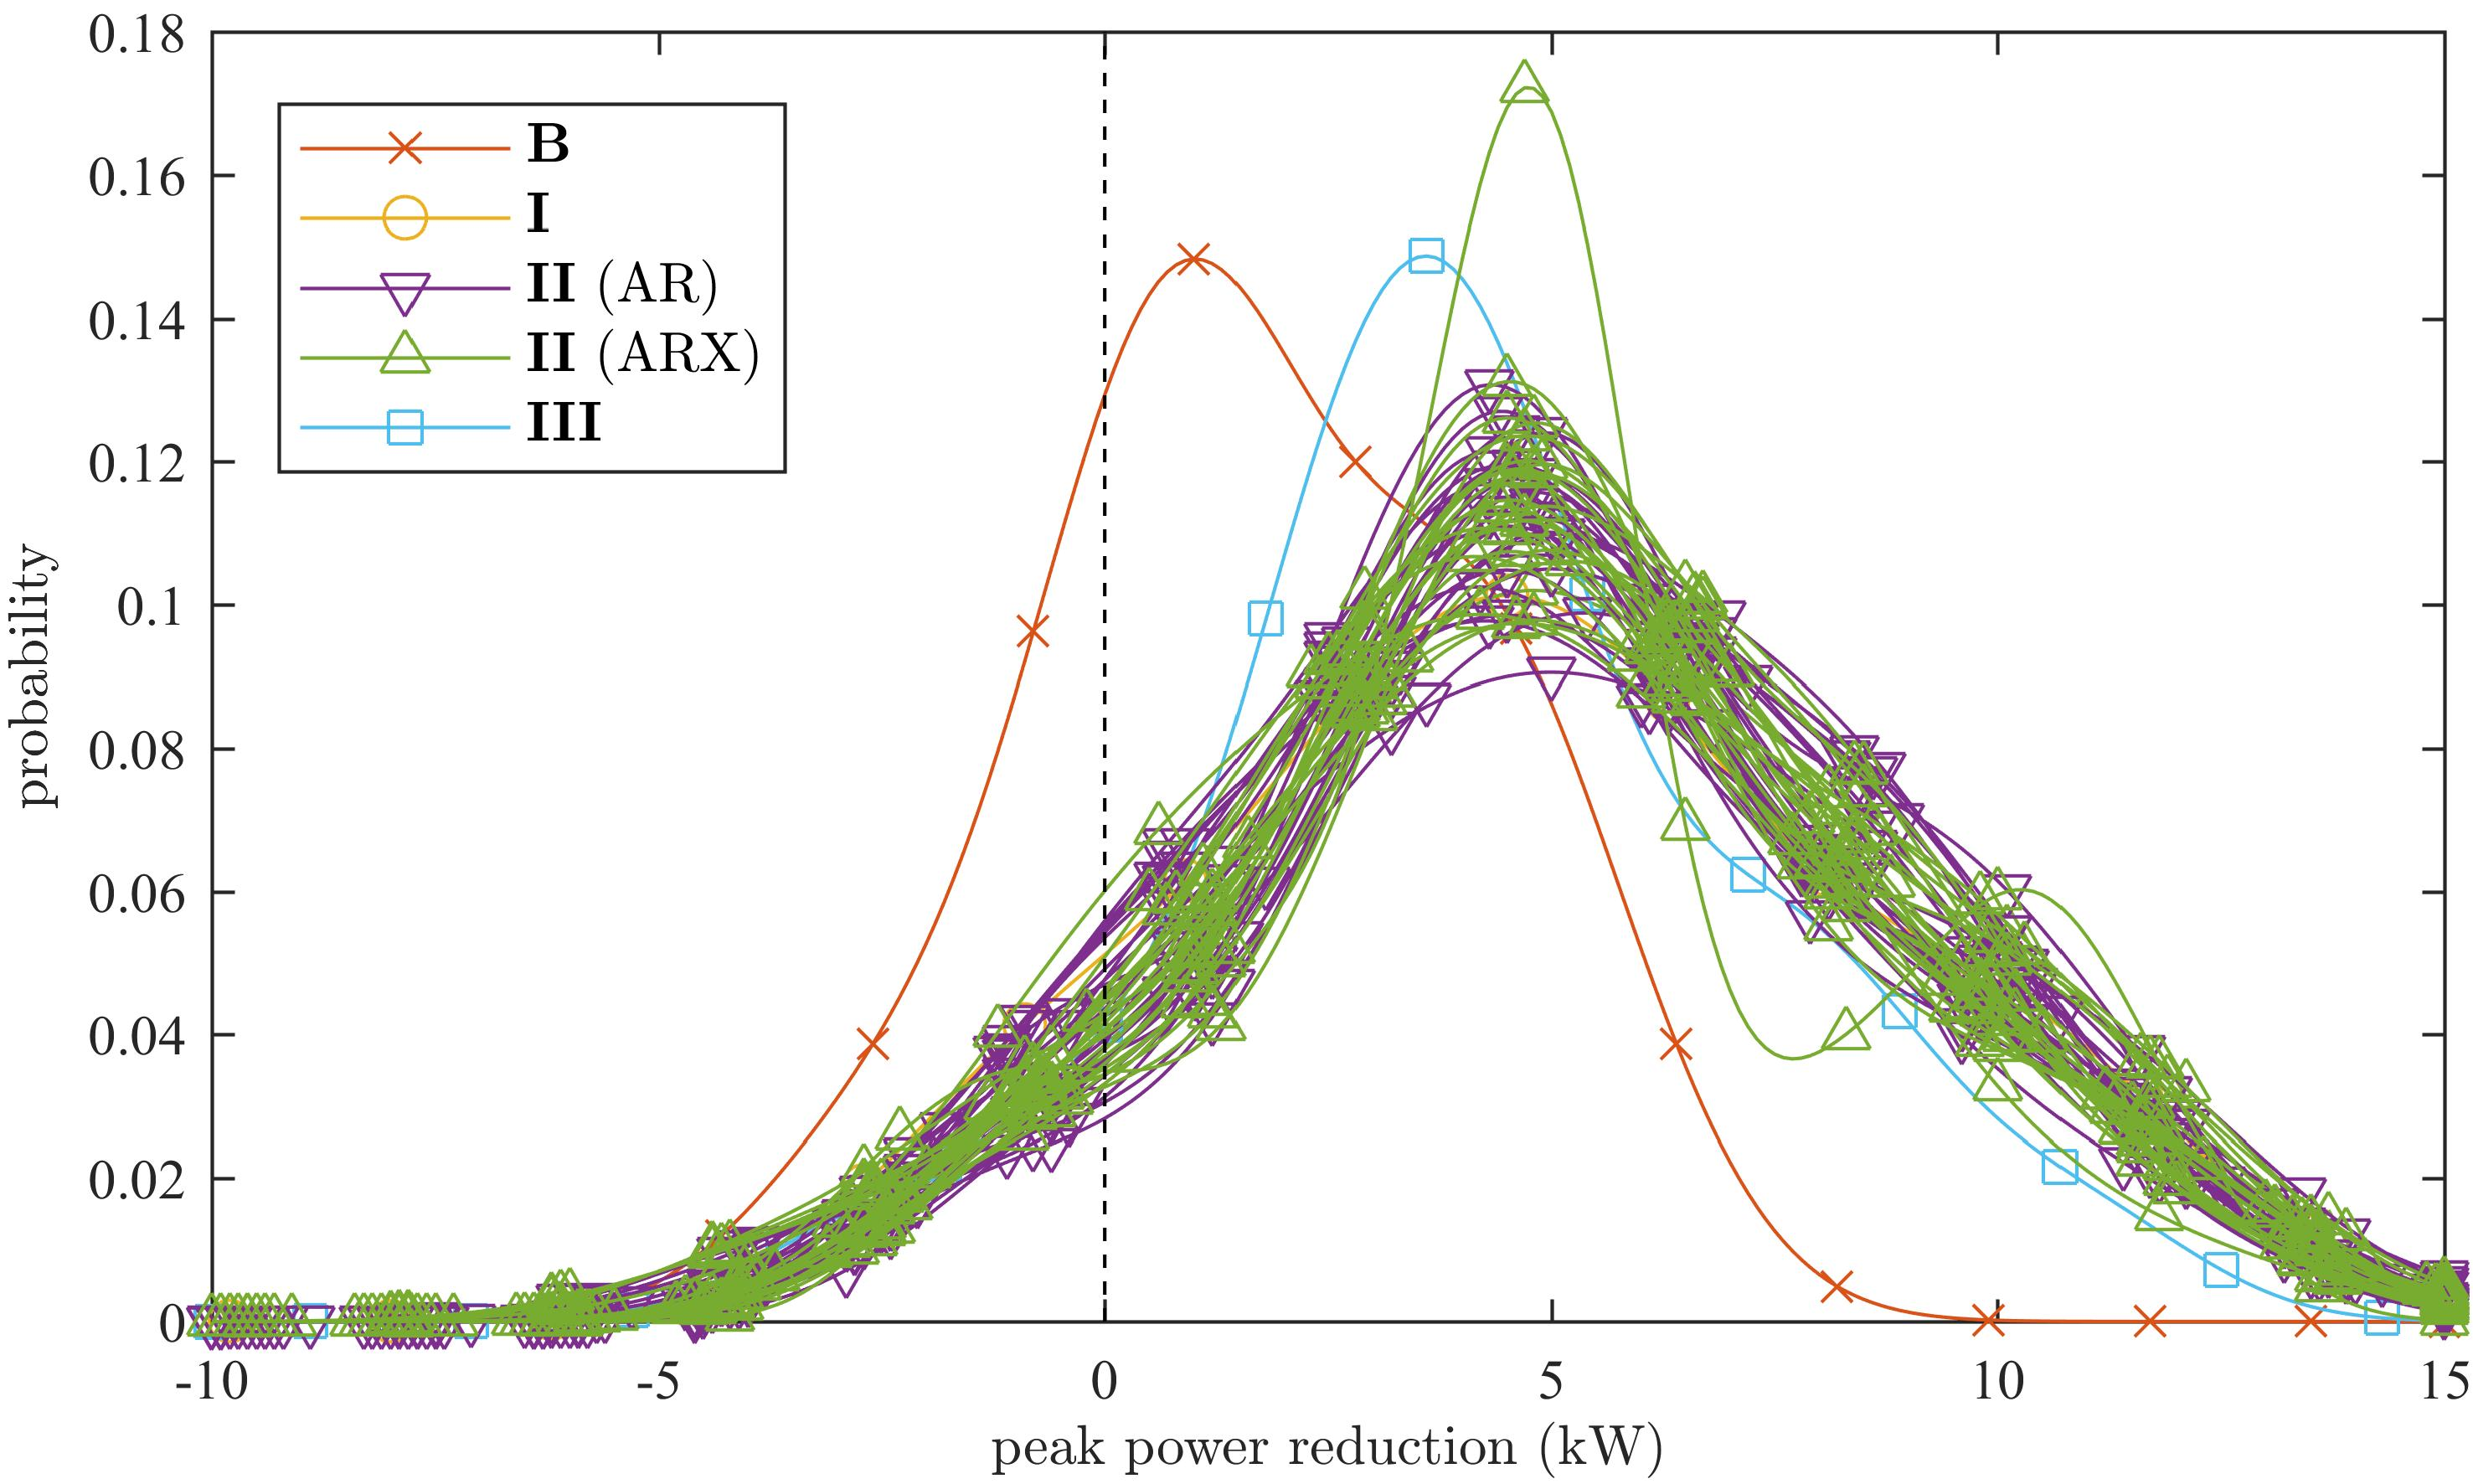
\includegraphics{_chapter2/fig/difference-pdf-1}
%	\subfloat[]{%
%		\includegraphics{_chapter2/fig/pdf-1}
%		\label{ch2:subfig:peak-pdf-1}
%	}
%	\vspace{0mm}
%	\subfloat[]{%
%		\includegraphics{_chapter2/fig/pdf-2}
%		\label{ch2:subfig:peak-pdf-2}
%	}
	\caption{Probability of peak load reduction for different prediction mechanisms and different AR/ARX model lentgths.}
	\label{ch2:fig:peak-pdf-multi-length}
\end{figure}

Similar to Figure \ref{ch2:fig:peak-diff-pdf}, Figure \ref{ch2:fig:peak-pdf-multi-length} shows the probability for the difference difference in peak power between the original case (\textbf{O}) and all other cases.
In this plot however, all PDFs for the different model lengths have been included (whilst the previous study only showed the inter-model means).
It can be seen, that both the AR and ARX case, \textbf{II}, performed noticeably better than the baseline case, \textbf{B}.
Despite the varying model length, all PDFs appear to peak around a reduction performance of 5kW.
Therefore, one may assume that the length of the chosen models does not significantly impact the results.

\begin{figure}\centering
	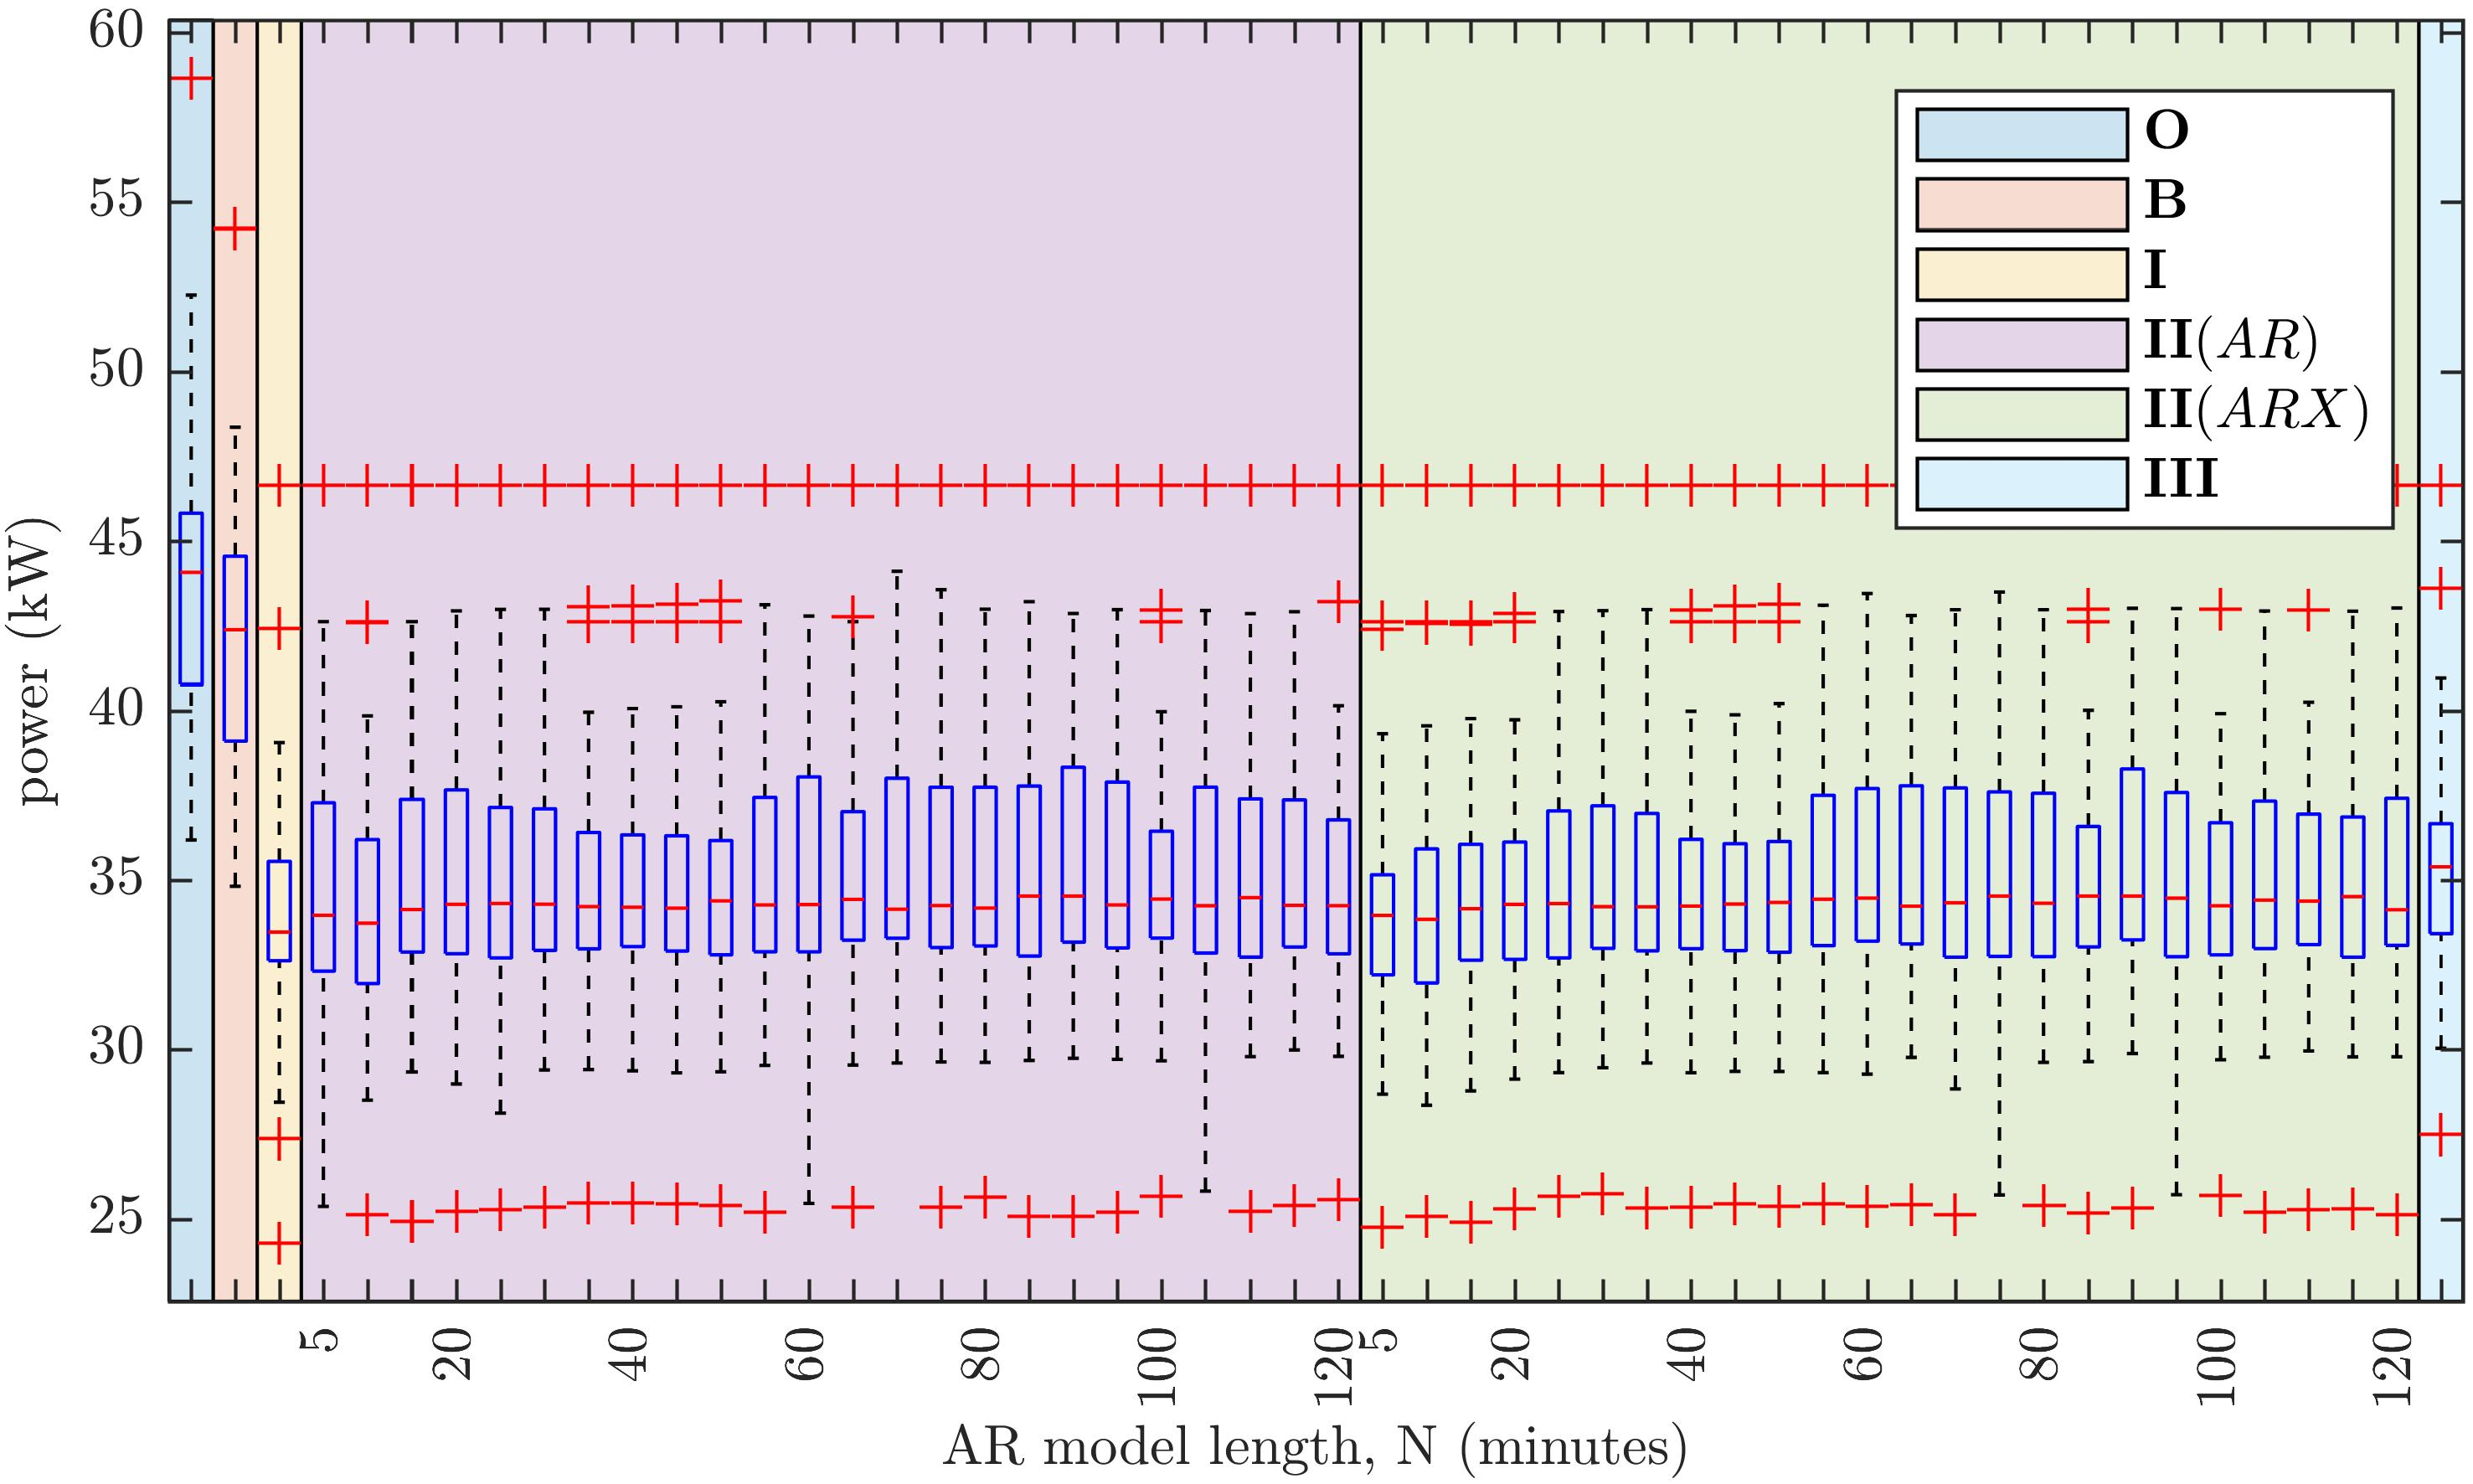
\includegraphics{_chapter2/fig/ar-length-peak-comparison-1}
%	\subfloat[]{%
%		\includegraphics{_chapter2/fig/pdf-1}
%		\label{ch2:subfig:peak-pdf-1}
%	}
%	\vspace{0mm}
%	\subfloat[]{%
%		\includegraphics{_chapter2/fig/pdf-2}
%		\label{ch2:subfig:peak-pdf-2}
%	}
	\caption{Visualisation of the peak power distribution for different AR/ARX model lengths.}
	\label{ch2:fig:boxplot-multi-length}
\end{figure}

This assumption is supported by the boxplots in Figure \ref{ch2:fig:boxplot-multi-length}, where the peak power distributions are visualised for all different model lengths and the six different case studies.
It can be seen, that the different AR/ARX model lengths, \textbf{II}, outperforms both the original and baseline cases, \textbf{O} and \textbf{B}, respectively.
Also, a certain variation in peak reduction performance can be observed, but no apparent trend.
Therefore, the assumption that the model length impacts the performance of the dynamic control is true, but the assumption that a longer model yields better results is not.
%The reason behind this fact is either based on the limitations of the dynamic control or on the AR/ARX models.
%However, assessing the complete catalogue of MPC lies beyond the scope of this thesis.



